\section{Additional Real-Data Figures}
\label{app:data_plots}

\subsection{Air Quality Data: ADMM Benchmark Fits}
\label{app:spod_admm}

The ADMM benchmark fits of Section~\ref{sec:app:spod}, and the detrended series
they produce, are collected here for comparison with
Figures~\ref{fig:spod_quantiles_pmala} and~\ref{fig:spod_detrended_pmala}.

\begin{figure}[!ht]
	\centering
	\begin{subfigure}{0.72\textwidth}
		\centering
		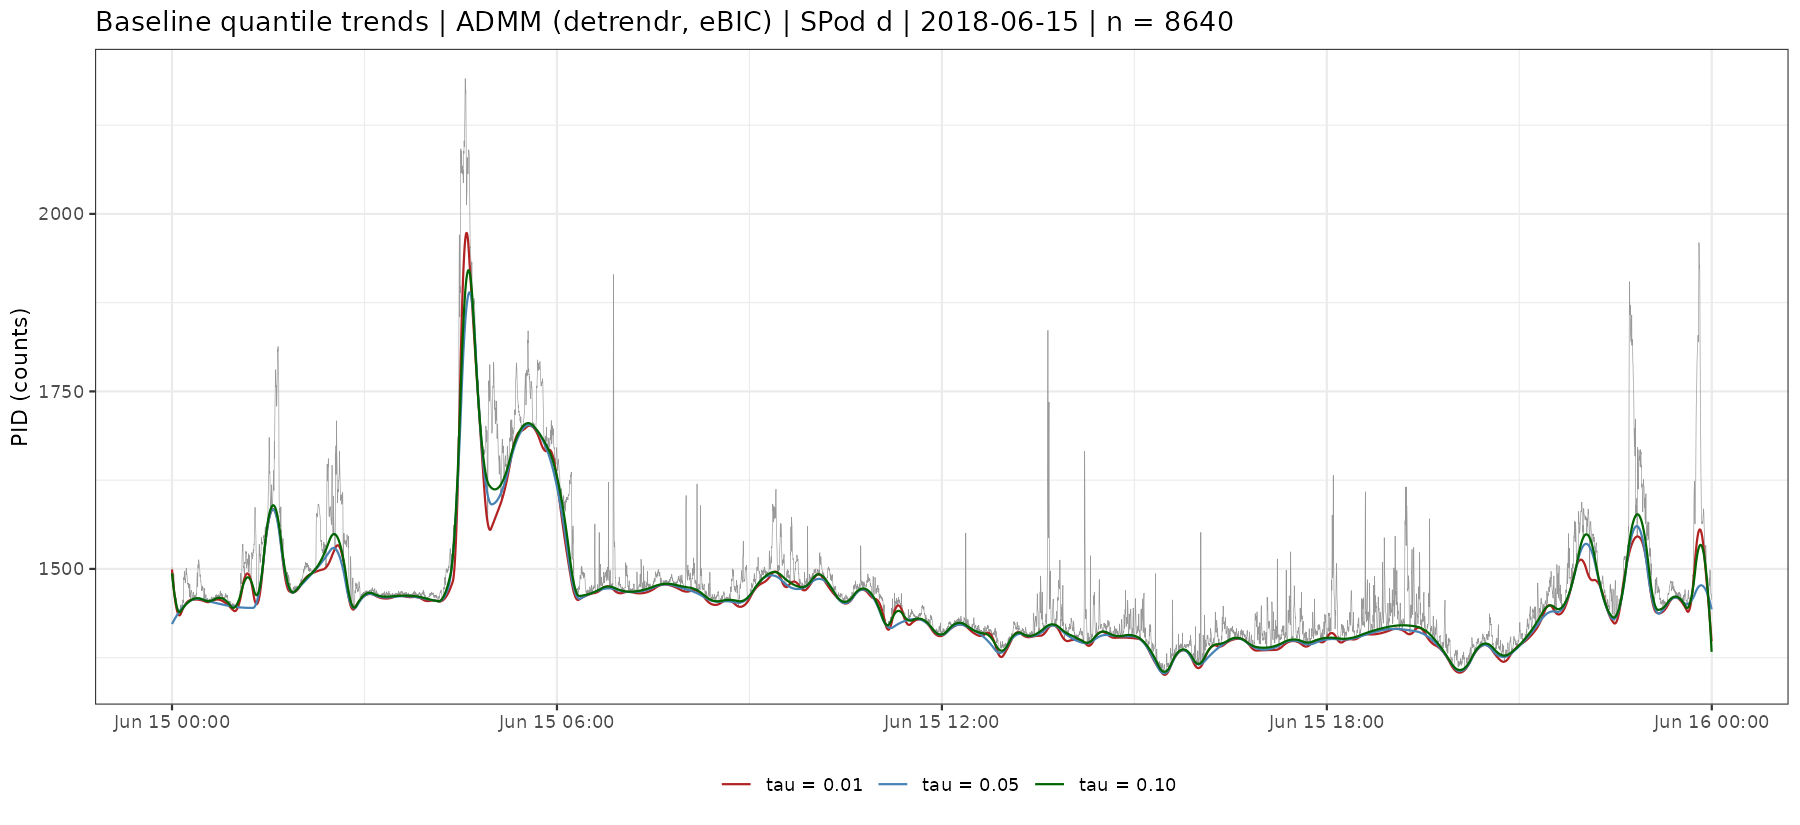
\includegraphics[width=\textwidth]{figures/spod_quantiles_admm}
		\caption{Baseline trends. Note the crossing of the $\tau = 0.01$ curve above
			the others at the 05:00 plume, induced by the small eBIC penalty at that level.}
		\label{fig:spod_quantiles_admm}
	\end{subfigure}
	\par\medskip
	\begin{subfigure}{0.72\textwidth}
		\centering
		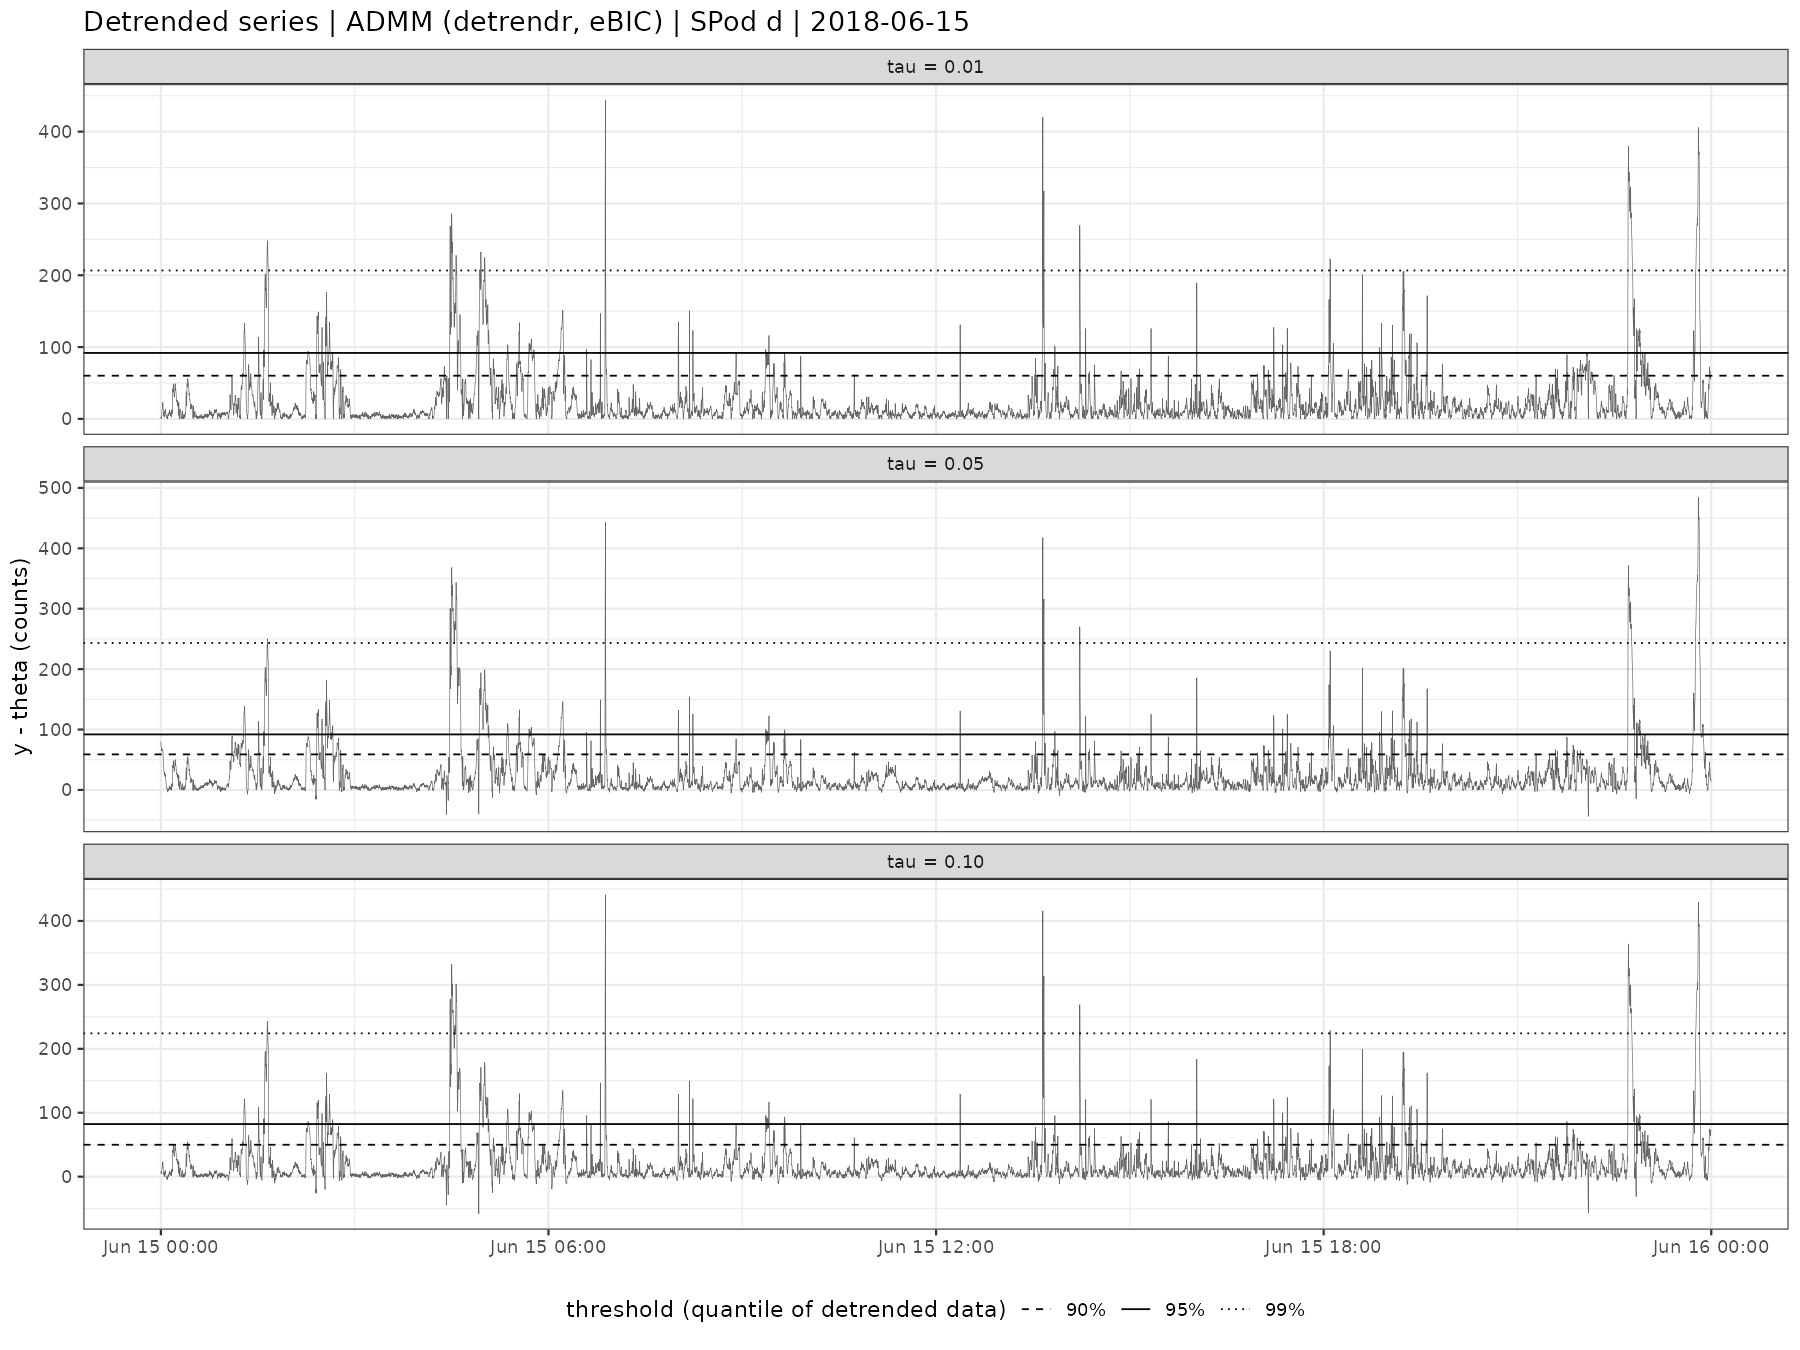
\includegraphics[width=\textwidth]{figures/spod_detrended_admm}
		\caption{Detrended series $\by - \widehat{\btheta}$, with the 90th (dashed),
			95th (solid), and 99th (dotted) empirical percentiles of the detrended data.}
		\label{fig:spod_detrended_admm}
	\end{subfigure}
	\caption{Air quality data: ADMM benchmark fits \citep{brantley2020baseline},
		$\lambda$ selected by eBIC, laid out as Figures~\ref{fig:spod_quantiles_pmala}
		and~\ref{fig:spod_detrended_pmala}.}
	\label{fig:spod_admm}
\end{figure}

\clearpage

\subsection{Munich Rent Data: Interior Quantile Levels}
\label{app:munich_interior}

Figures~\ref{fig:munich_pmala_305070} and~\ref{fig:munich_onizuka_305070} complete the Munich analysis of Section~\ref{sec:app:munich} with the fits at $\tau \in \{0.3, 0.5, 0.7\}$, obtained under exactly the settings described there ($k = 1$; $6{,}000$ iterations, $1{,}000$ burn-in; one independent chain per level).

\begin{figure}[htbp]
	\centering
	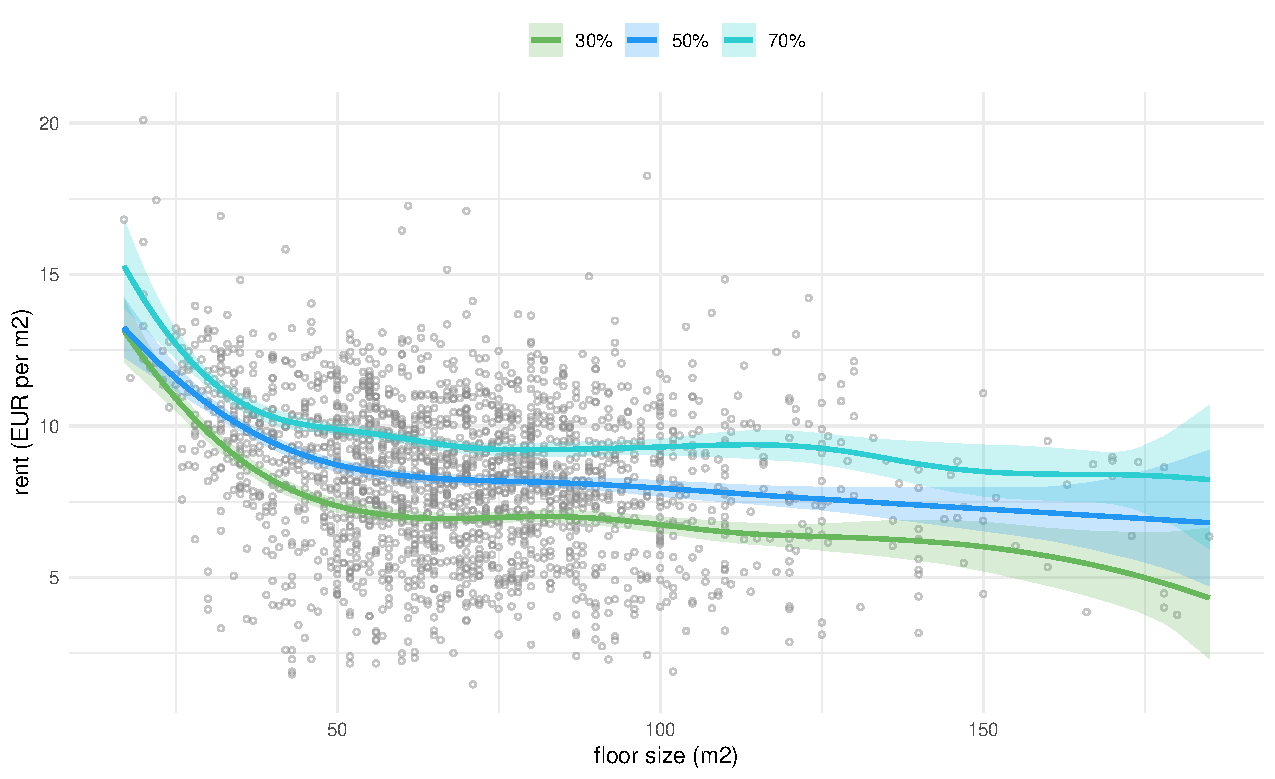
\includegraphics[width=0.75\textwidth]{figures/munich_pmala_q30_q50_q70}
	\caption{Munich rent data: $30\%$, $50\%$, and $70\%$ conditional quantiles estimated by the individual P-MALA/Gibbs sampler with $k = 1$. Solid curves are posterior means and ribbons are $95\%$ pointwise credible intervals; grey circles are the observations.}
	\label{fig:munich_pmala_305070}
\end{figure}

\begin{figure}[htbp]
	\centering
	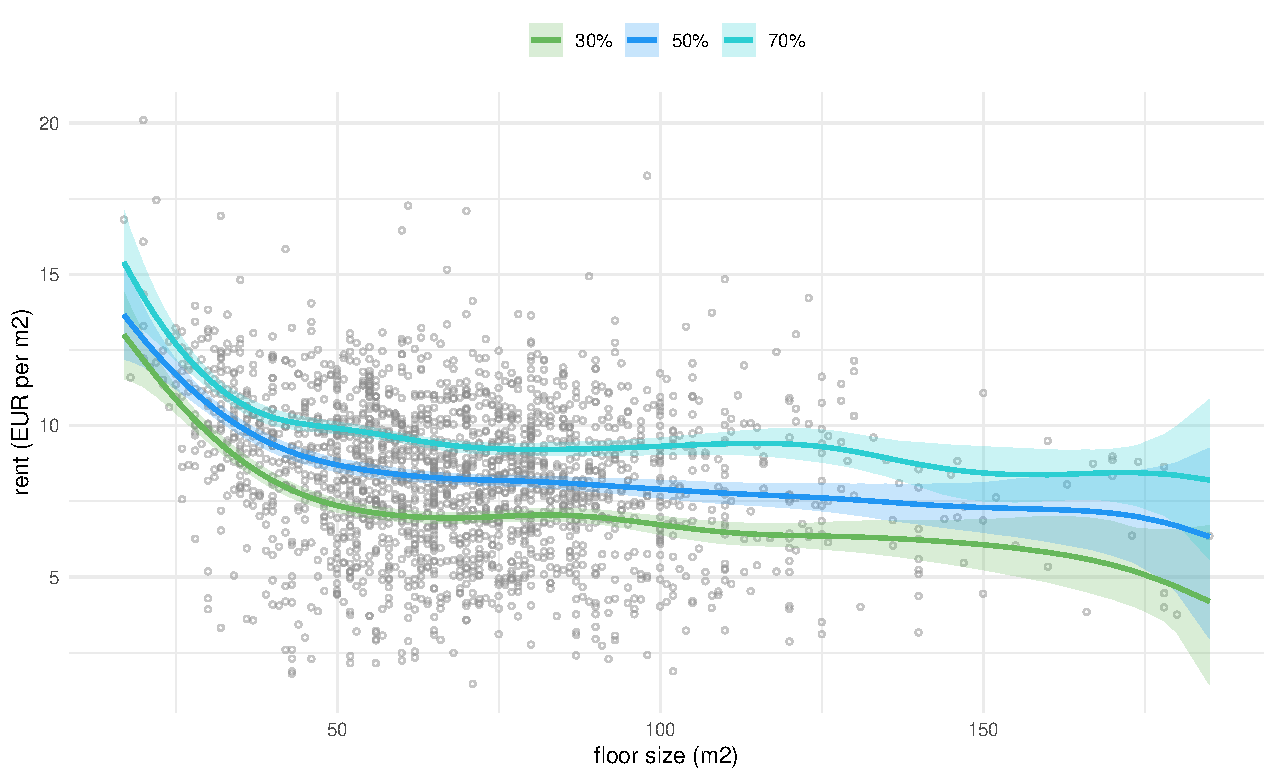
\includegraphics[width=0.75\textwidth]{figures/munich_onizuka_q30_q50_q70}
	\caption{Munich rent data: $30\%$, $50\%$, and $70\%$ conditional quantiles estimated by the horseshoe sampler of \citet{onizuka2024fast} (MCMC mode) with $k = 1$, under the same layout as Figure~\ref{fig:munich_pmala_305070}.}
	\label{fig:munich_onizuka_305070}
\end{figure}

% ----------------------------------------------------------------------------
% Diagnostics from the earlier (k = 2, 60,000-iteration) Nile and Munich runs.
% Parked here until the diagnostics are regenerated for the k = 1 fits above;
% the figure files are still in figures/.
% ----------------------------------------------------------------------------
\iffalse
This appendix collects all plots for the real-data applications.  The fits
use the unchanged application P-MALA/Gibbs sampler for 60,000 iterations, with
10,000 burn-in iterations and thinning by 10.

\begin{figure}[p]
	\centering
	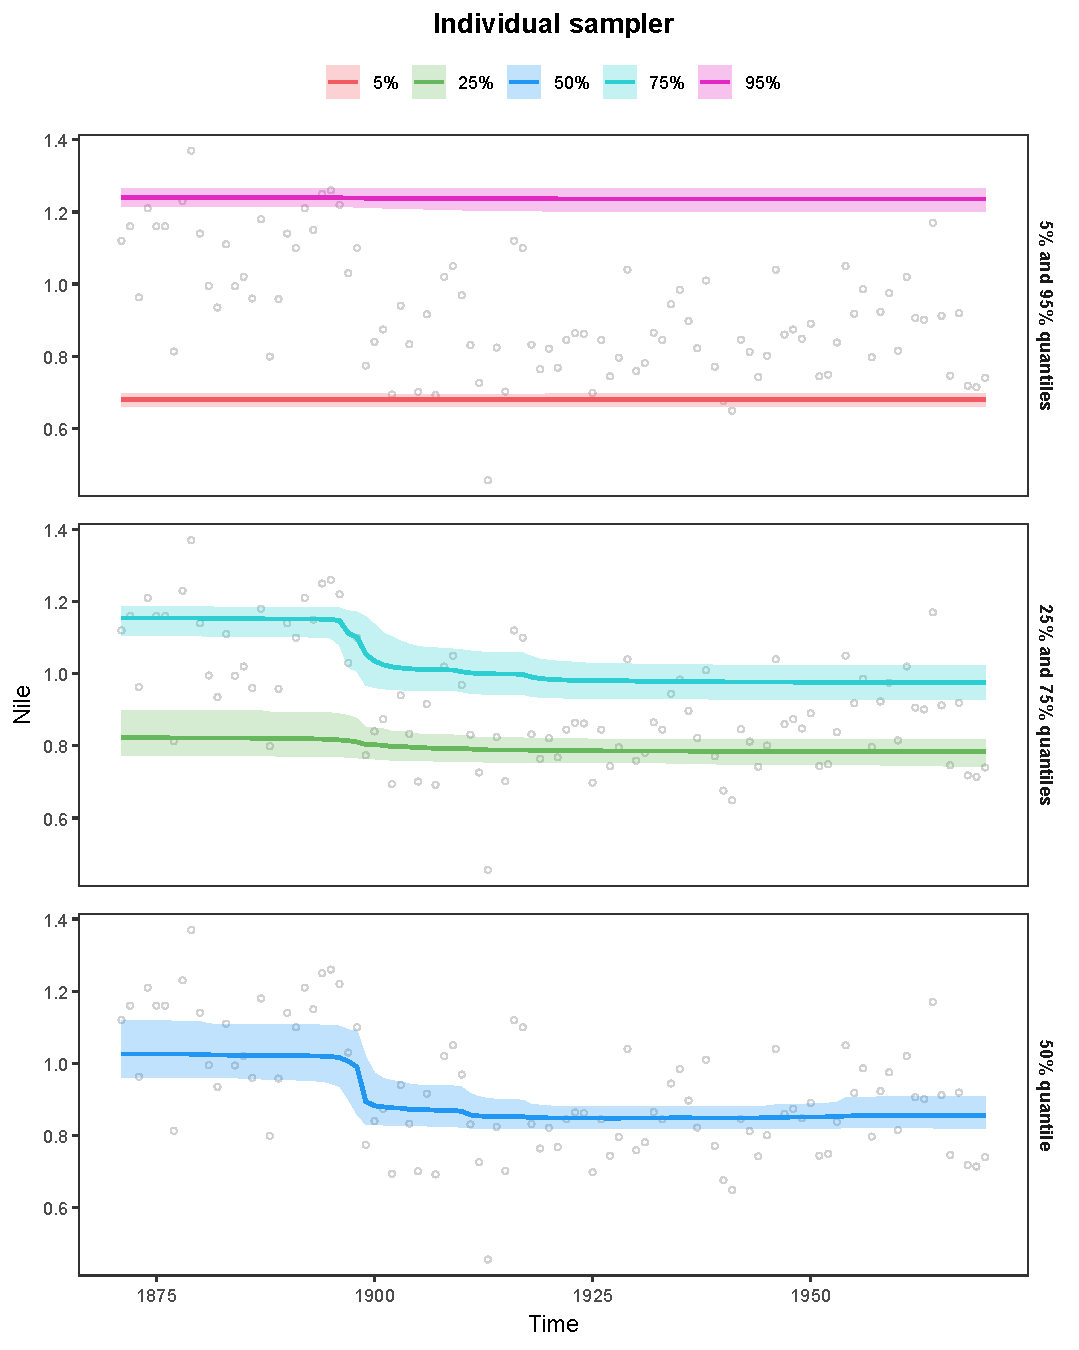
\includegraphics[width=0.75\textwidth,height=0.82\textheight,keepaspectratio]
	{figures/nile_individual_sampler}
	\caption{Individual P-MALA/Gibbs fits for the Nile data.  Solid curves are
		posterior means and ribbons are 95\% pointwise credible intervals from the
		5,000 retained draws.  Grey circles are the rescaled observations.}
	\label{fig:nile}
\end{figure}

\begin{figure}[p]
	\centering
	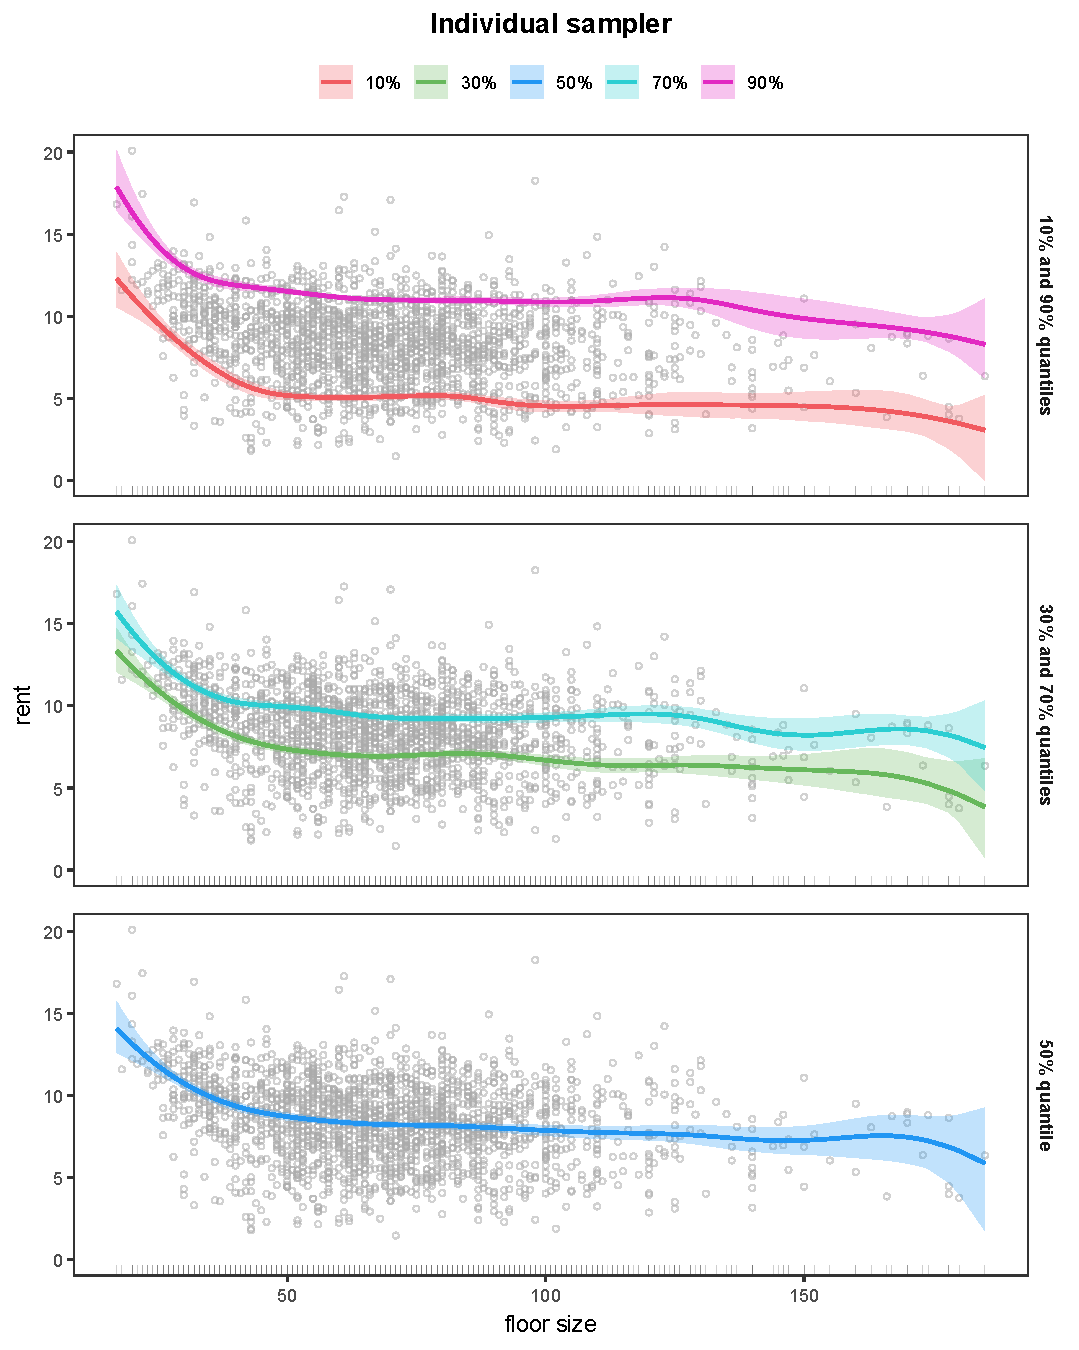
\includegraphics[width=0.75\textwidth,height=0.82\textheight,keepaspectratio]
	{figures/munich_individual_sampler}
	\caption{Individual P-MALA/Gibbs fits for Munich rent per square metre.
		Curves and ribbons are posterior means and 95\% pointwise credible intervals.
		The rug marks the observed floor sizes.}
	\label{fig:munich}
\end{figure}

\begin{figure}[p]
	\centering
	\begin{subfigure}{0.75\textwidth}
		\centering
		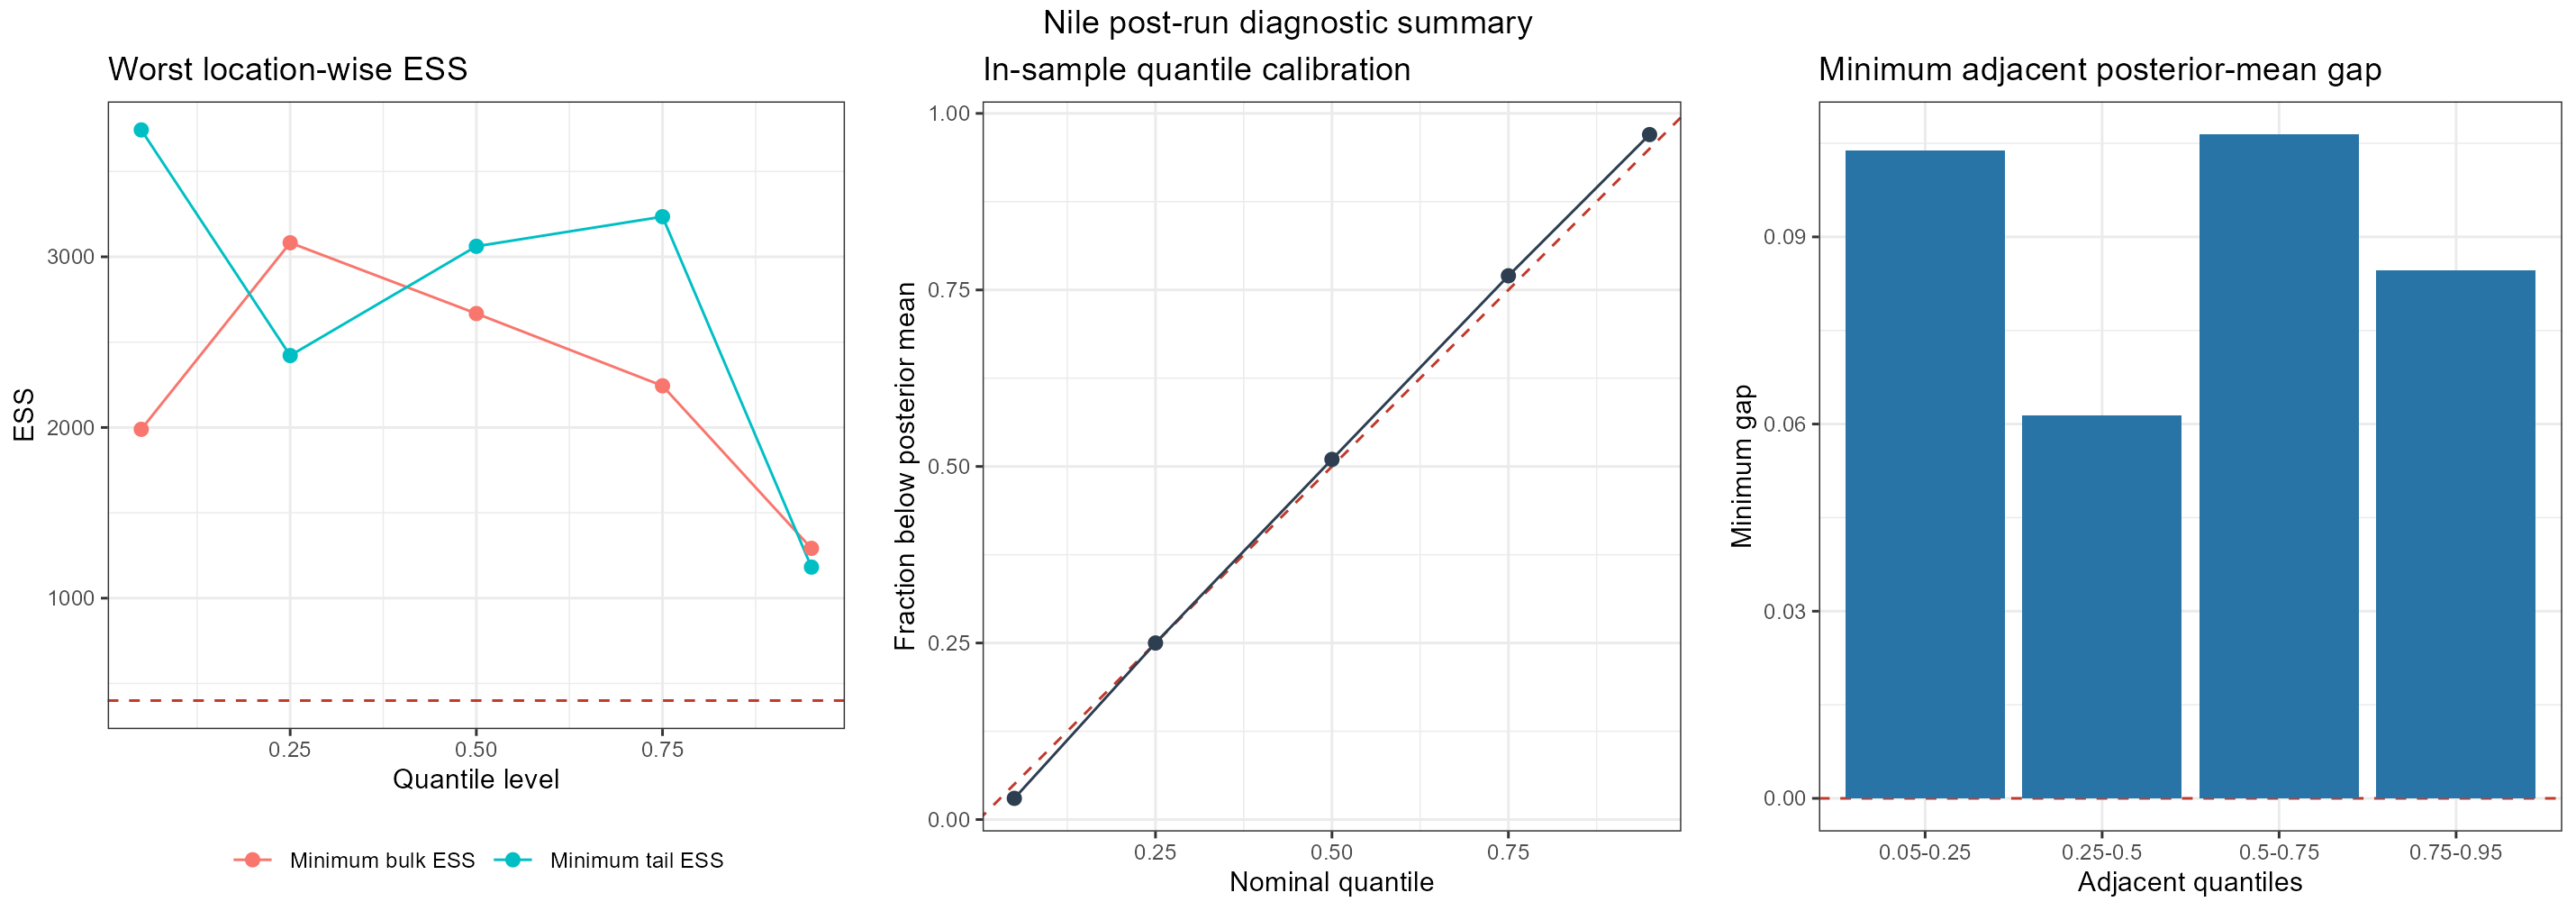
\includegraphics[width=\textwidth]{figures/nile_diagnostic_summary}
		\caption{Nile.}
	\end{subfigure}
	\par\medskip
	\begin{subfigure}{0.75\textwidth}
		\centering
		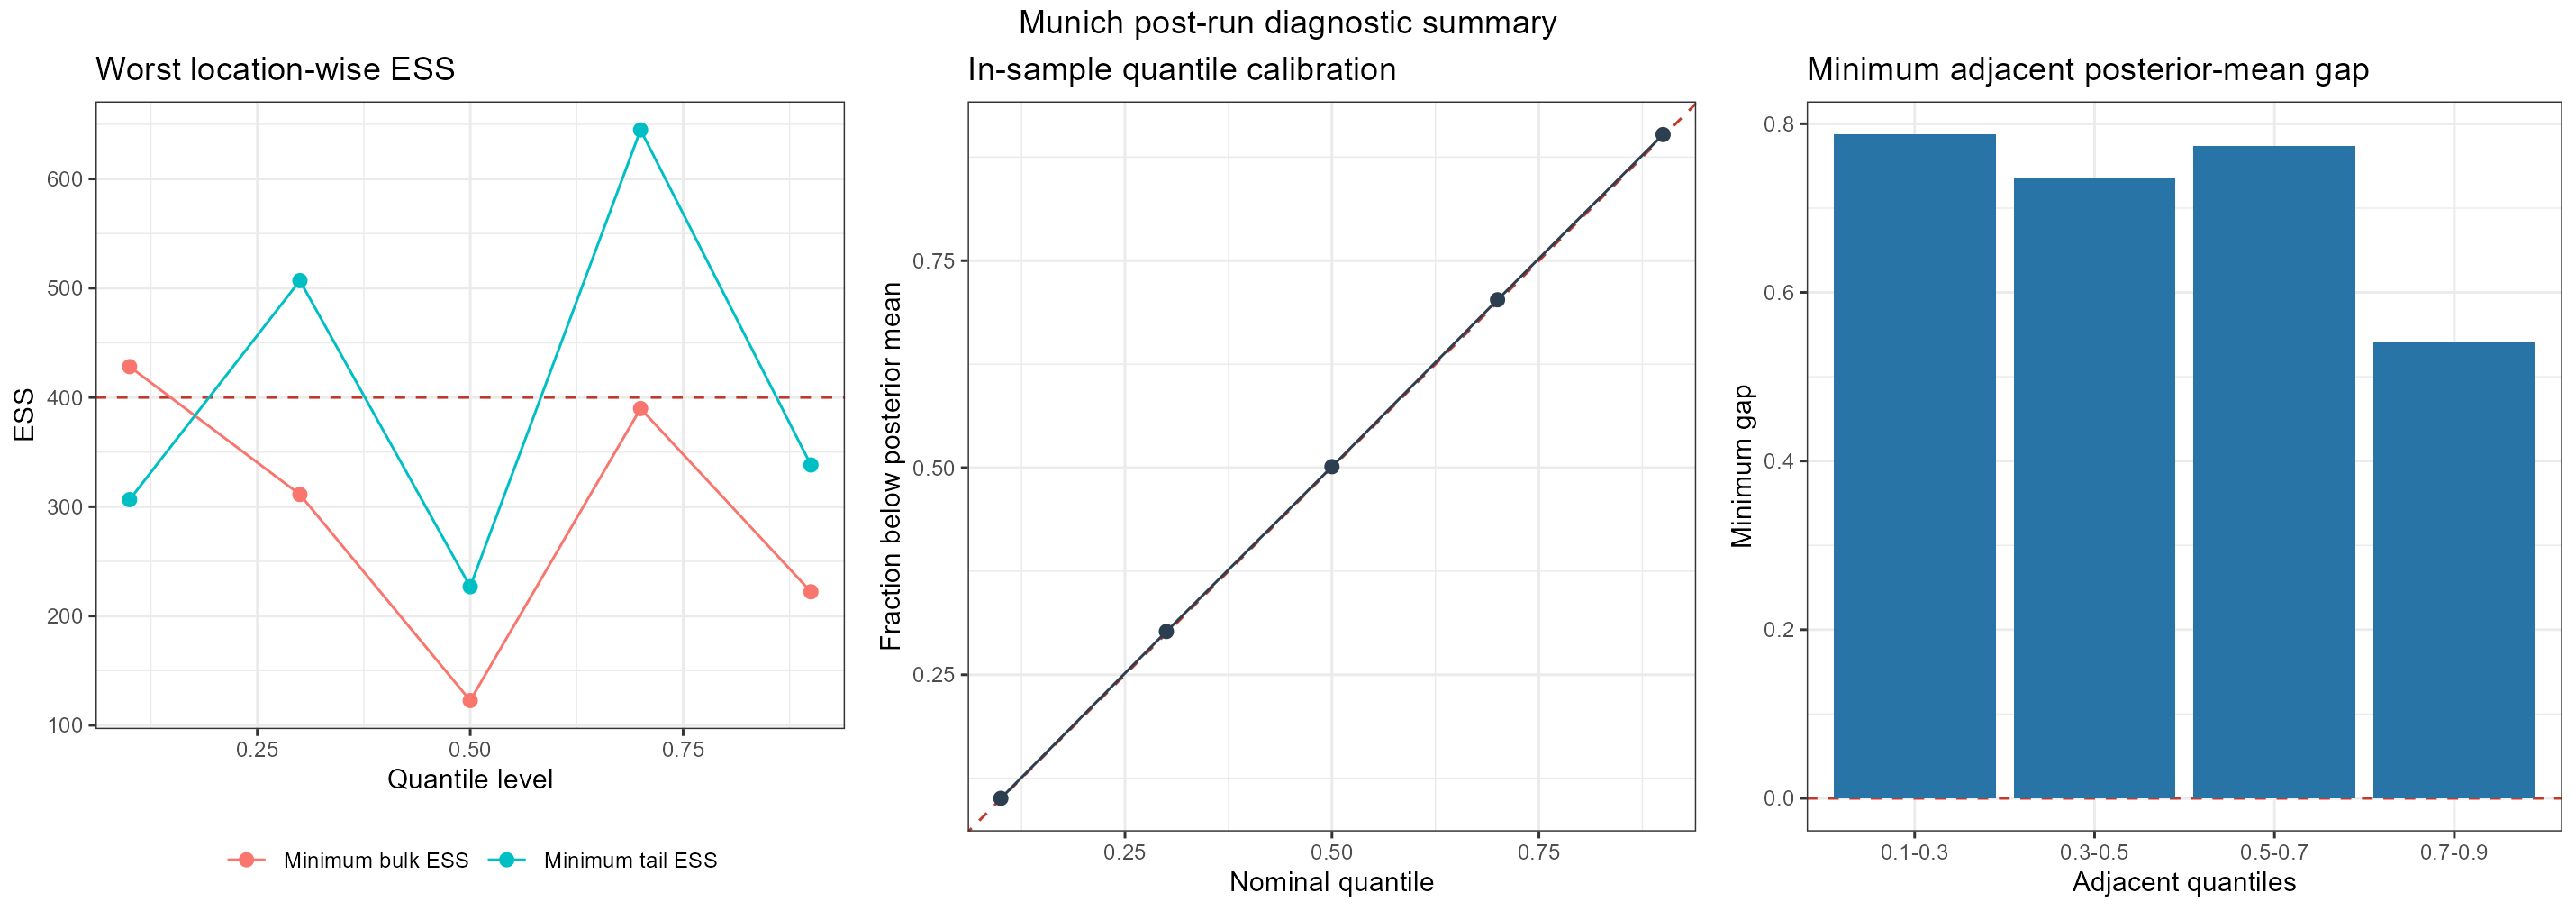
\includegraphics[width=\textwidth]{figures/munich_diagnostic_summary}
		\caption{Munich.}
	\end{subfigure}
	\caption{Post-run summaries: worst location-wise bulk and tail ESS, in-sample
		calibration, and minimum gap between adjacent posterior-mean curves.  The ESS
		reference line is 400 and the calibration reference is the identity line.}
	\label{fig:app_diag_summary}
\end{figure}

\begin{figure}[p]
	\centering
	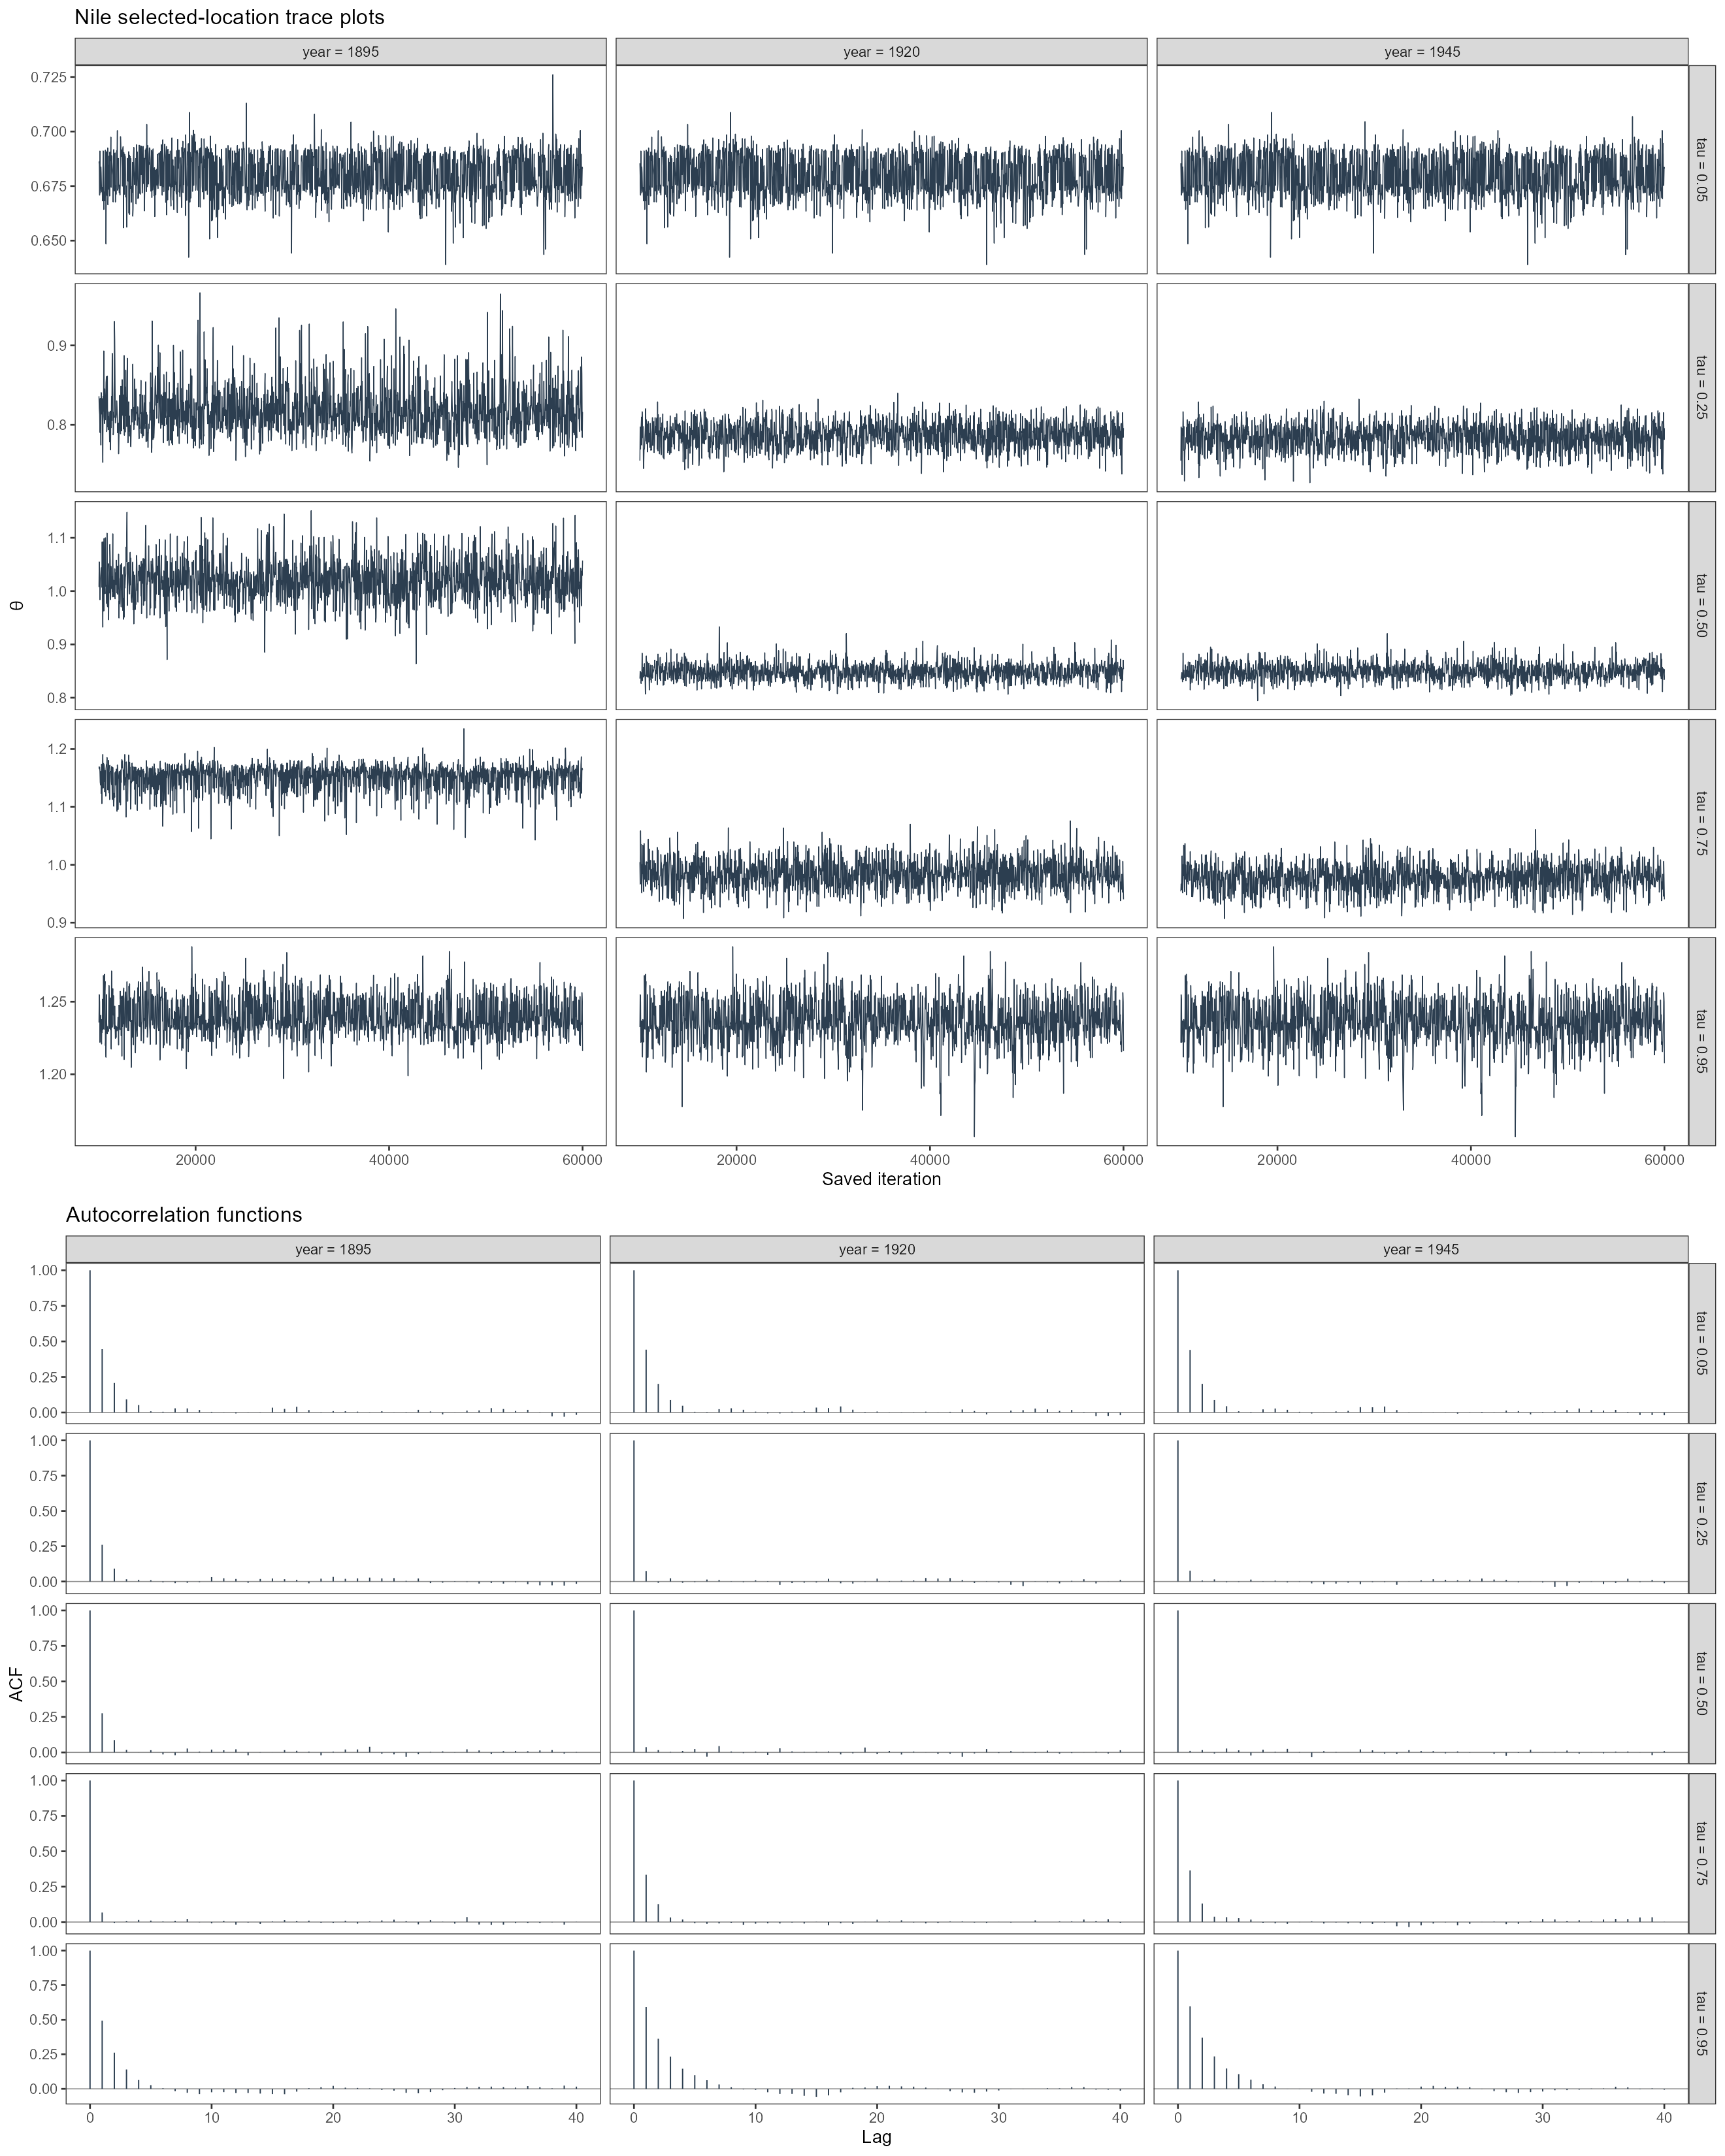
\includegraphics[width=0.75\textwidth,height=0.88\textheight,keepaspectratio]
	{figures/nile_trace_acf_diagnostics}
	\caption{Nile coefficient trace and autocorrelation diagnostics at
		representative years 1895, 1920, and 1945 for all five quantile levels.  The
		horizontal scale of the trace panels is the original Gibbs iteration, so
		adjacent plotted values are ten iterations apart.}
	\label{fig:nile_trace_acf}
\end{figure}

\begin{figure}[p]
	\centering
	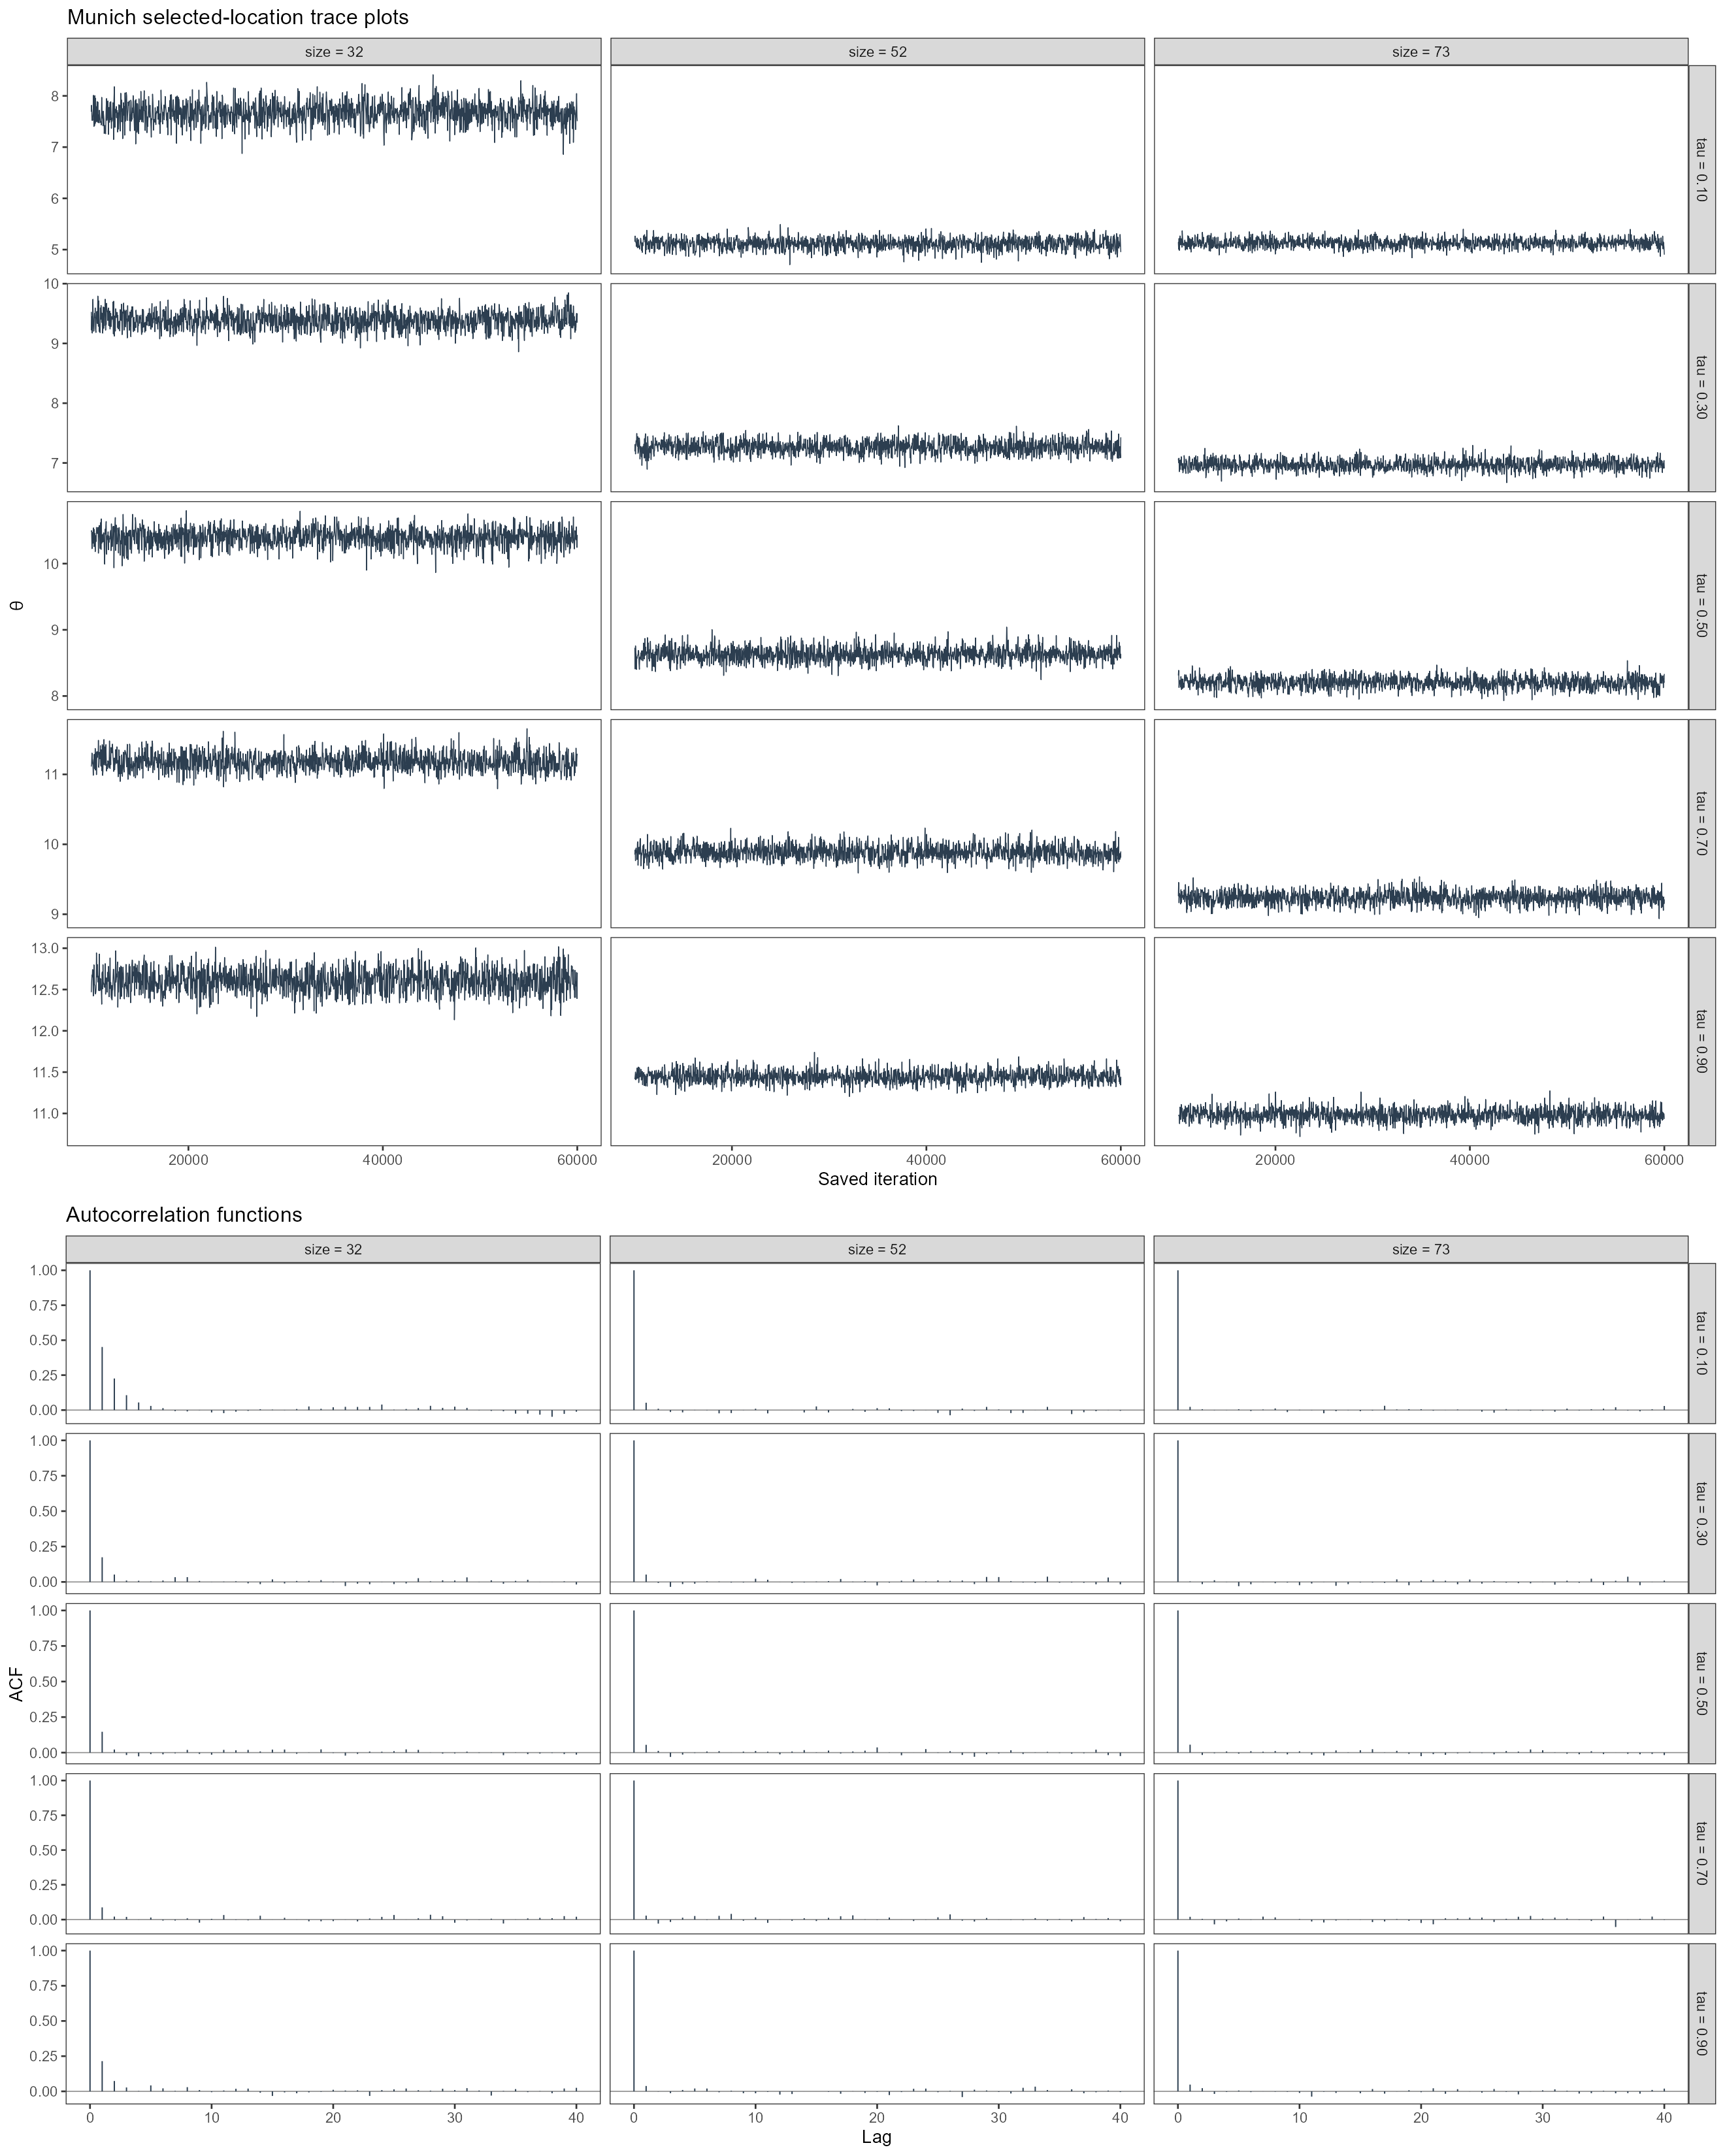
\includegraphics[width=0.75\textwidth,height=0.88\textheight,keepaspectratio]
	{figures/munich_trace_acf_diagnostics}
	\caption{Munich coefficient trace and autocorrelation diagnostics at
		representative floor sizes 32, 52, and 73 square metres.  The traces show
		stable levels, while the ACFs document the remaining quantile- and
		location-dependent persistence.}
	\label{fig:munich_trace_acf}
\end{figure}

\begin{figure}[p]
	\centering
	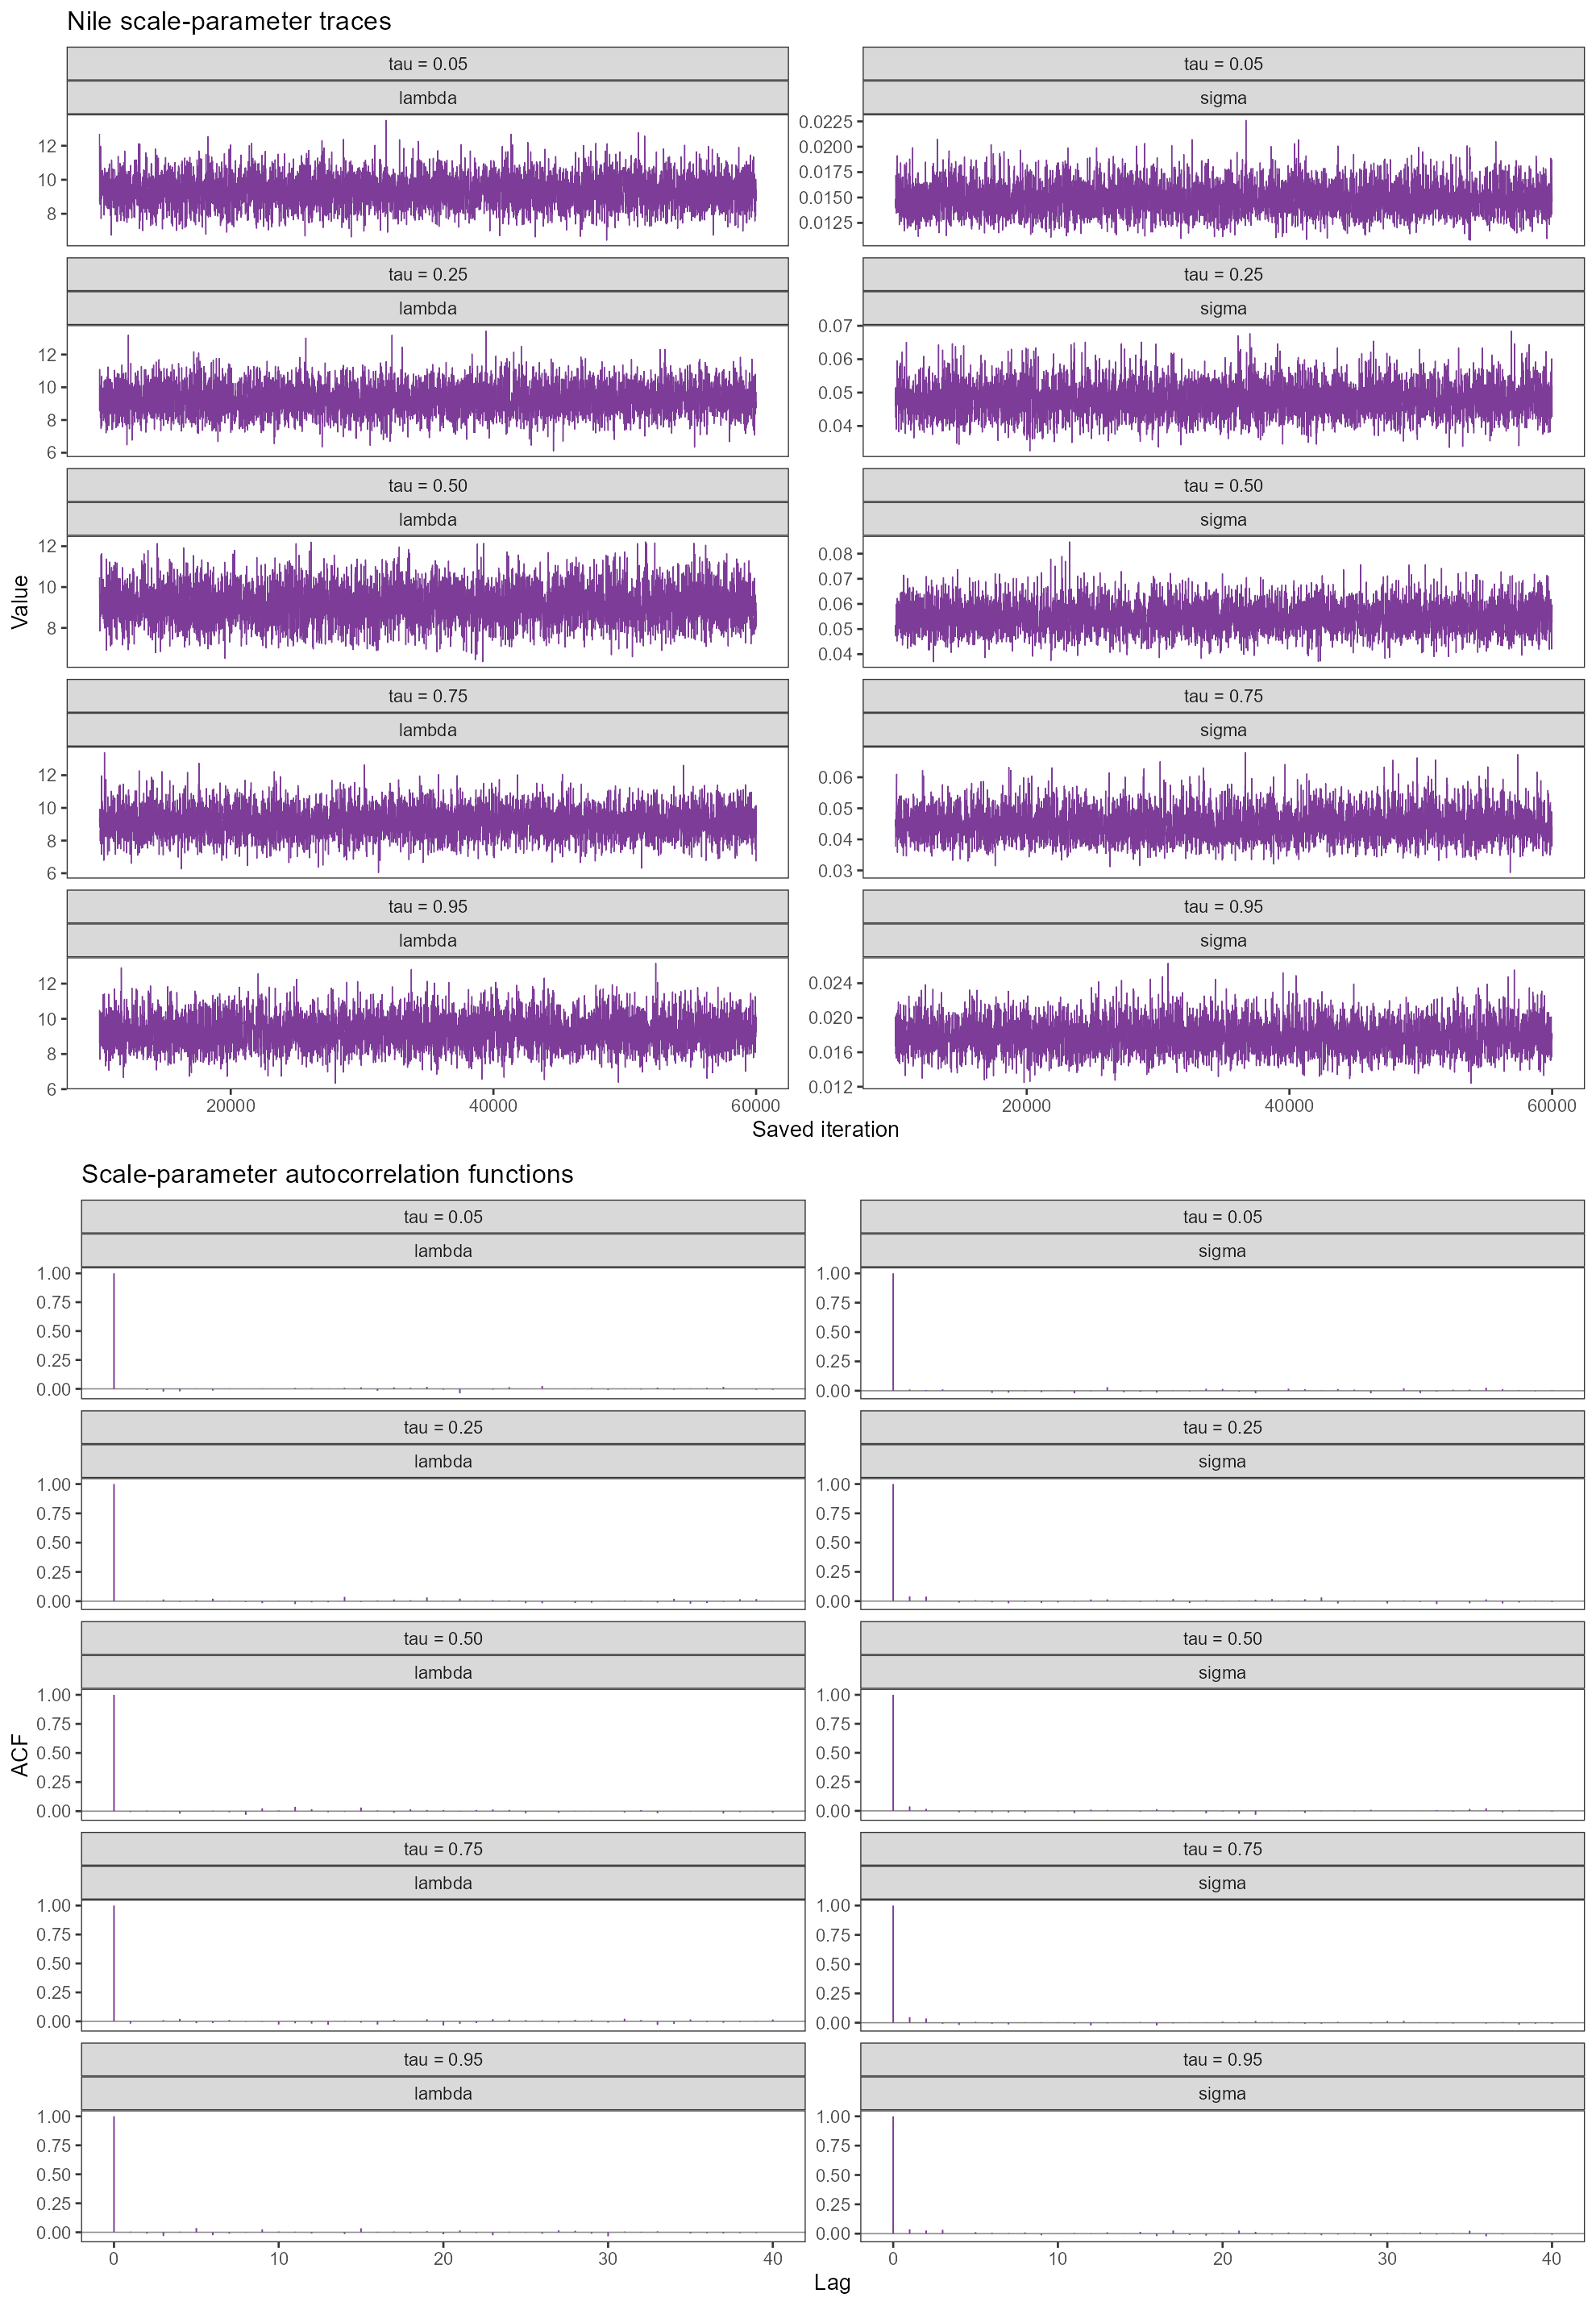
\includegraphics[width=0.75\textwidth,height=0.88\textheight,keepaspectratio]
	{figures/nile_scale_trace_acf_diagnostics}
	\caption{Nile trace and autocorrelation diagnostics for \(\lambda\) and
		\(\sigma\).  Both scale-parameter chains mix rapidly and show no visible
		drift.}
	\label{fig:nile_scale_trace_acf}
\end{figure}

\begin{figure}[p]
	\centering
	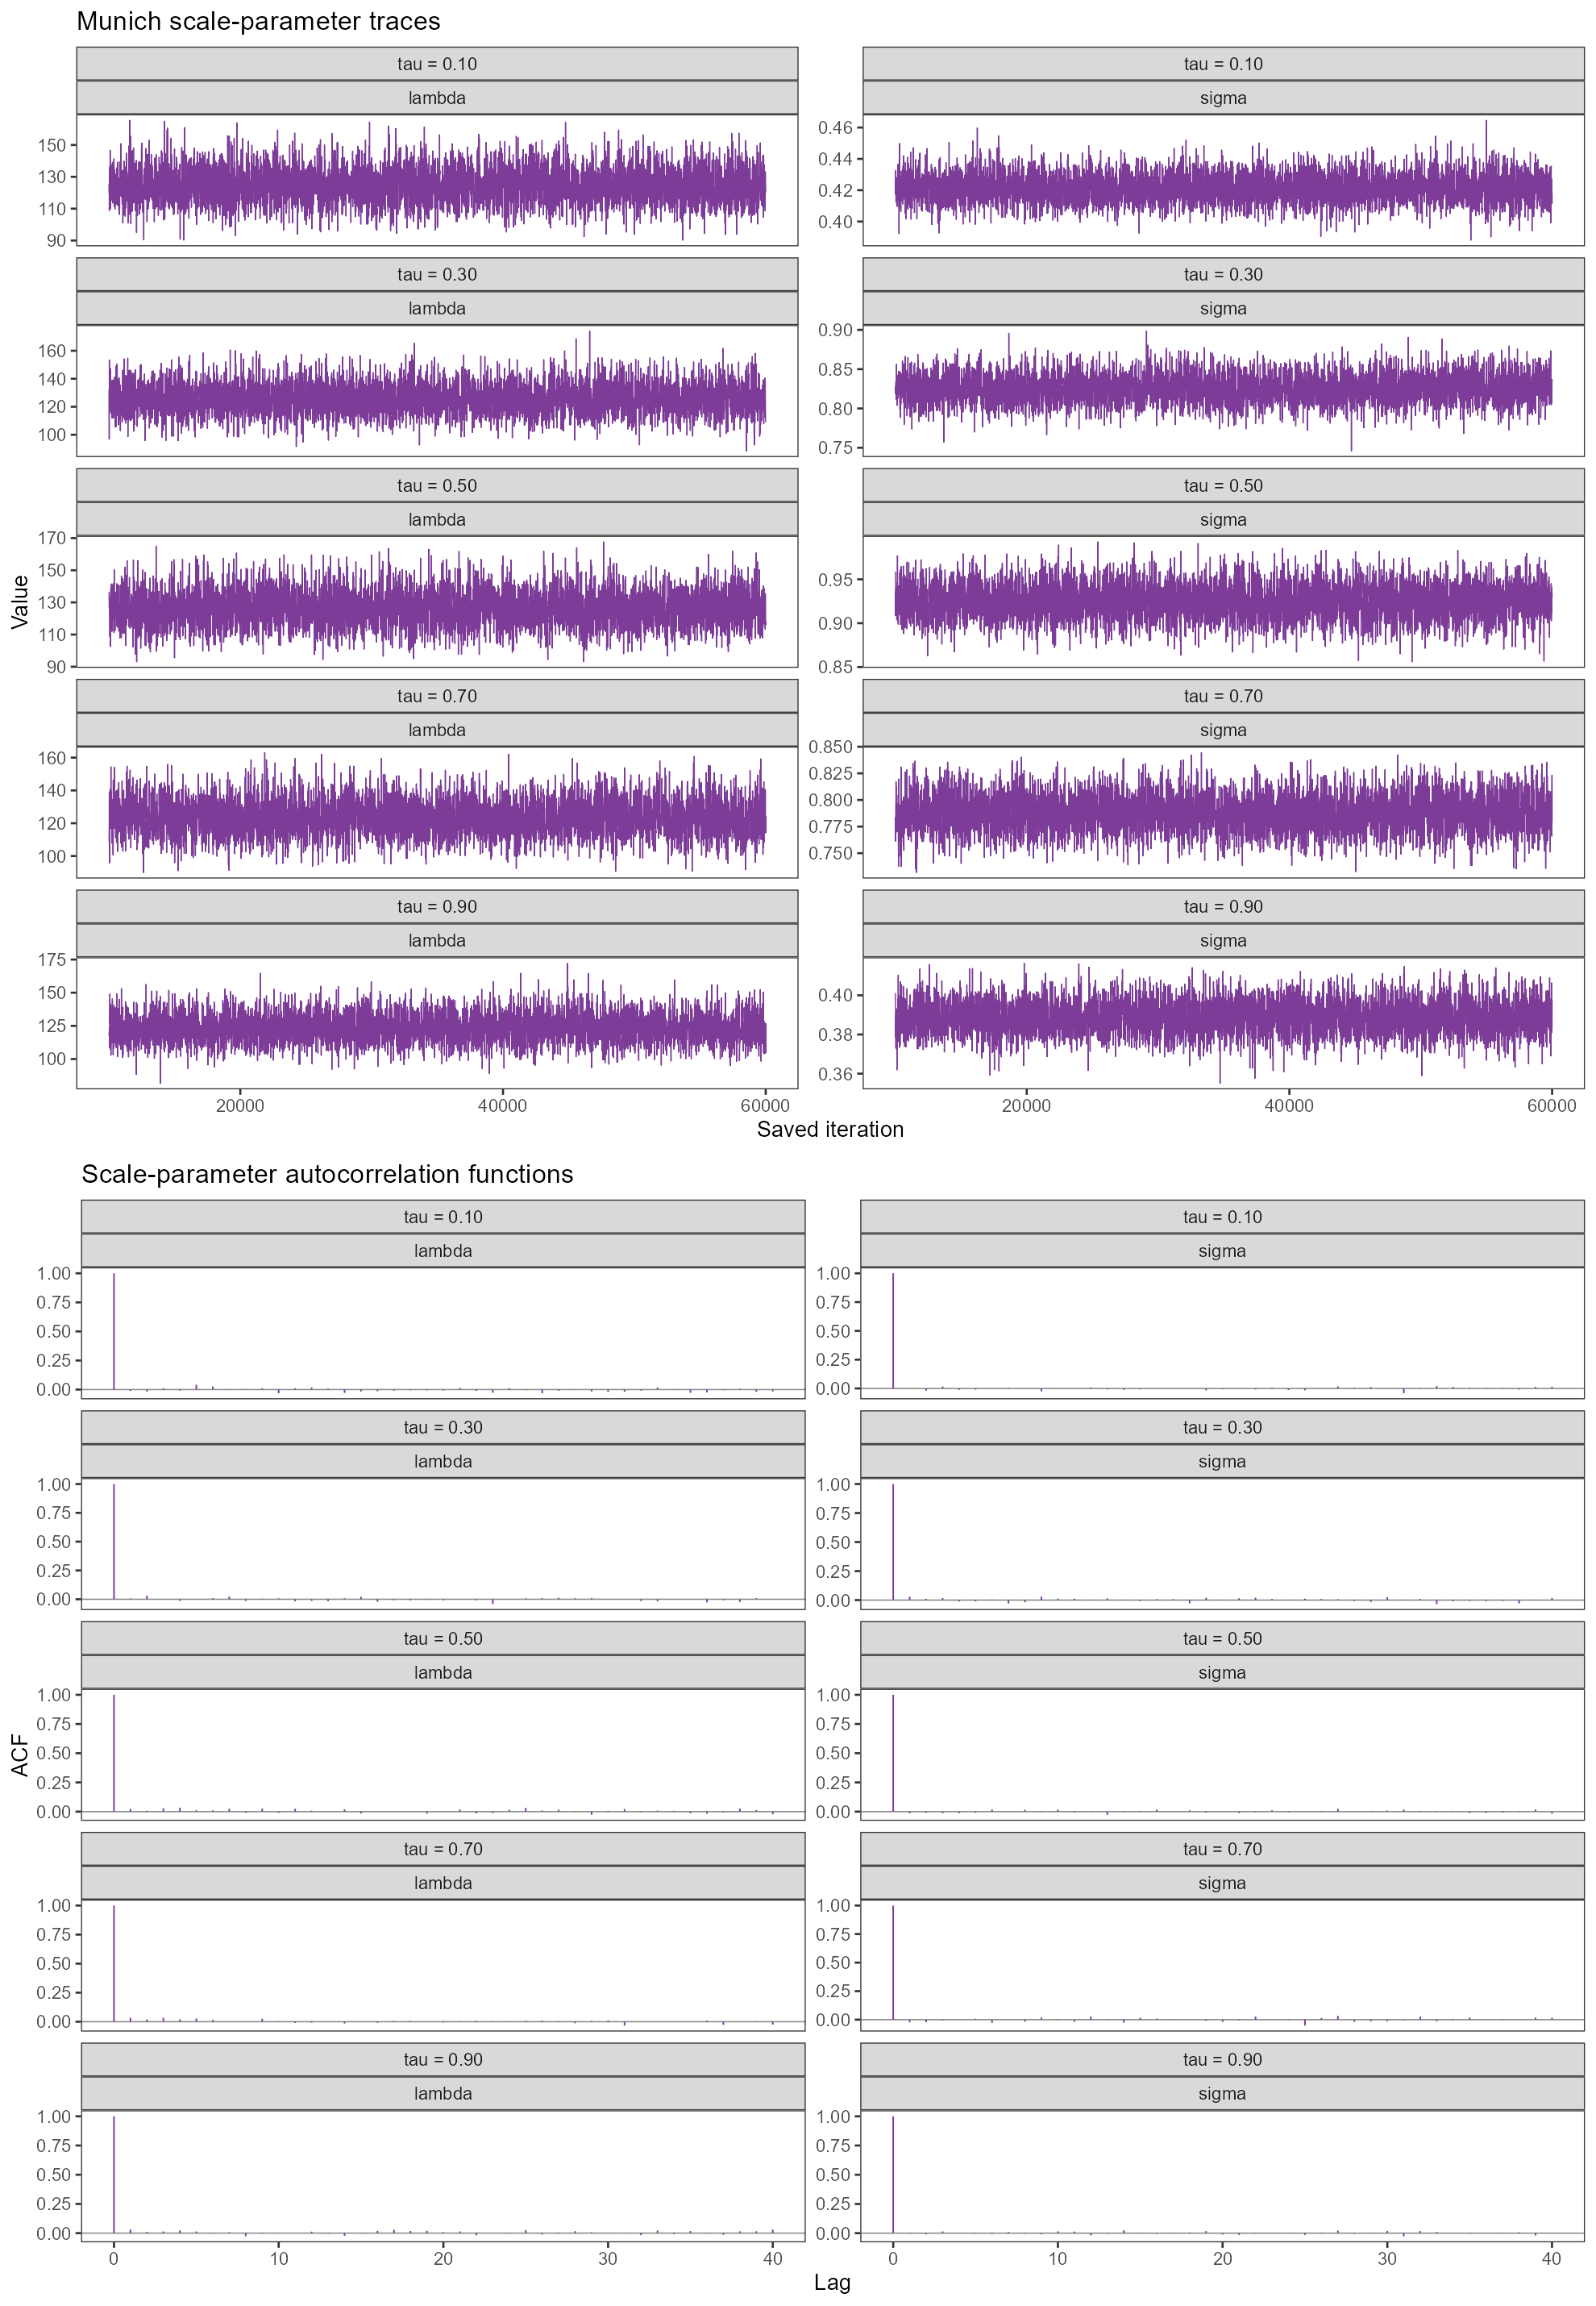
\includegraphics[width=0.75\textwidth,height=0.88\textheight,keepaspectratio]
	{figures/munich_scale_trace_acf_diagnostics}
	\caption{Munich trace and autocorrelation diagnostics for \(\lambda\) and
		\(\sigma\).  The low autocorrelations show that the slowest Munich mixing is
		concentrated in trend coefficients rather than the scale parameters.}
	\label{fig:munich_scale_trace_acf}
\end{figure}

\begin{figure}[p]
	\centering
	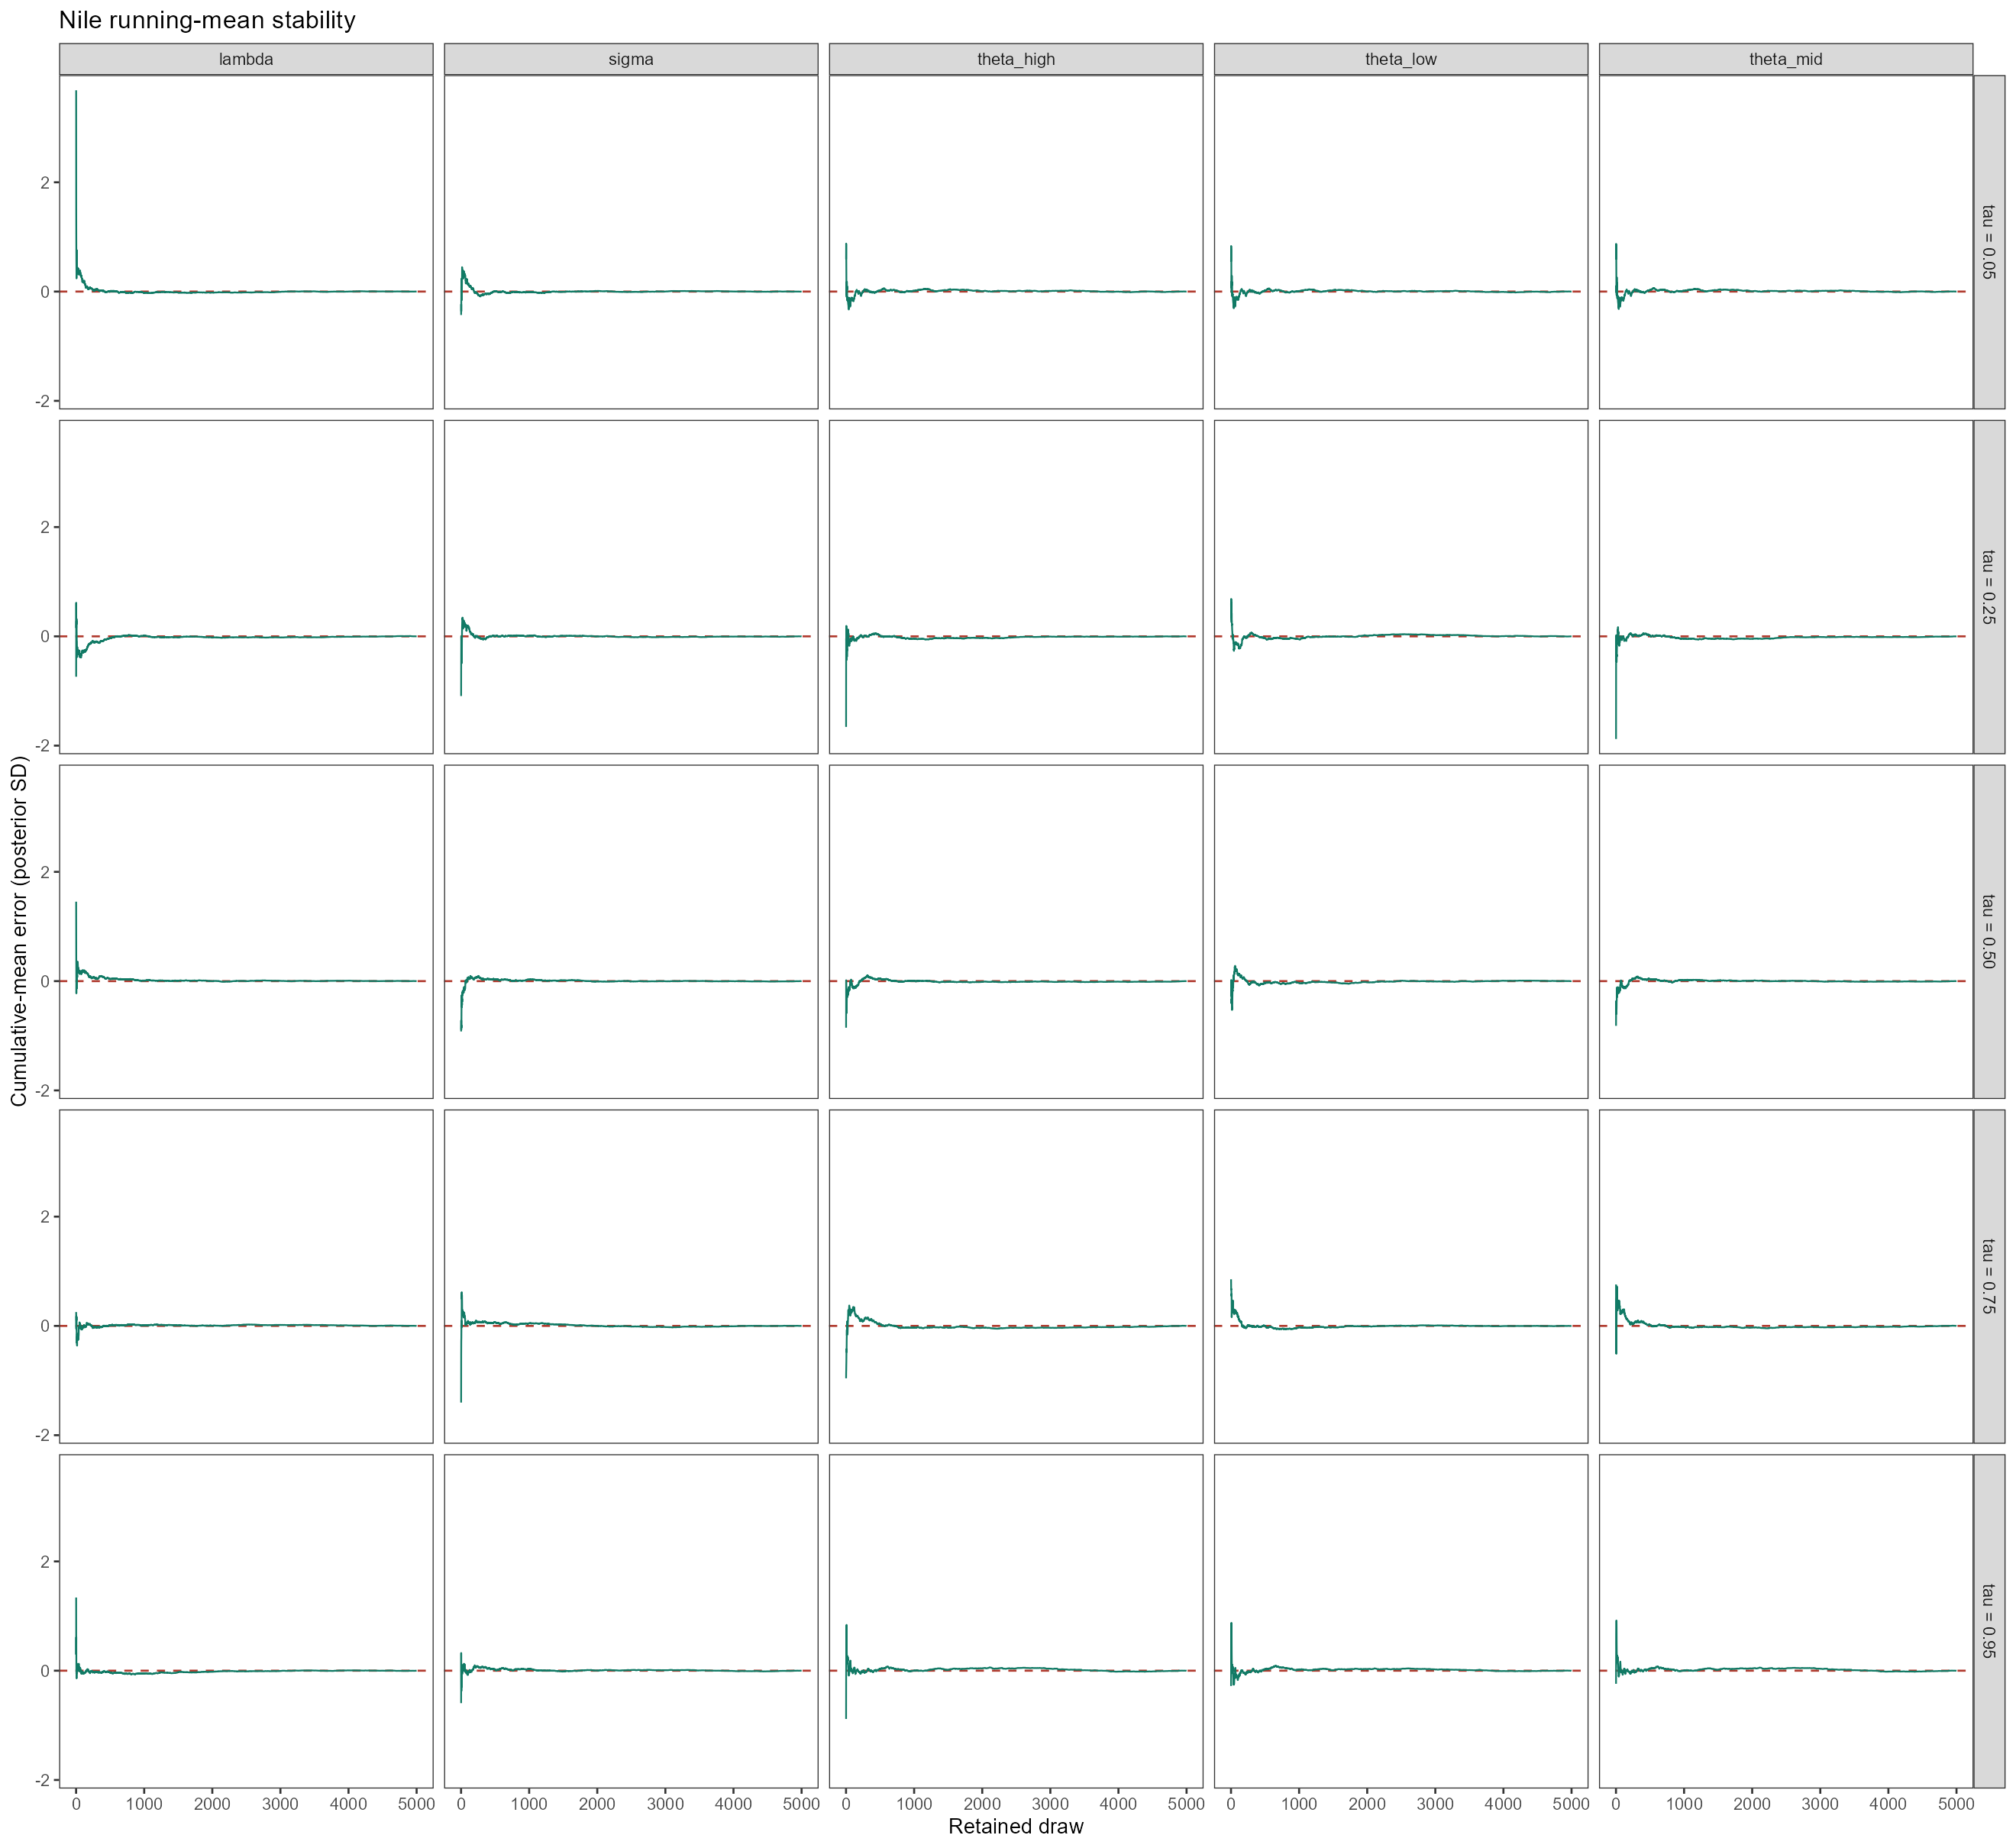
\includegraphics[width=0.75\textwidth,height=0.88\textheight,keepaspectratio]
	{figures/nile_running_mean_stability}
	\caption{Nile standardized cumulative-mean diagnostics.  Each curve is the
		cumulative mean minus its final posterior mean, divided by the posterior
		standard deviation; the dashed line is zero.}
	\label{fig:nile_running_mean}
\end{figure}

\begin{figure}[p]
	\centering
	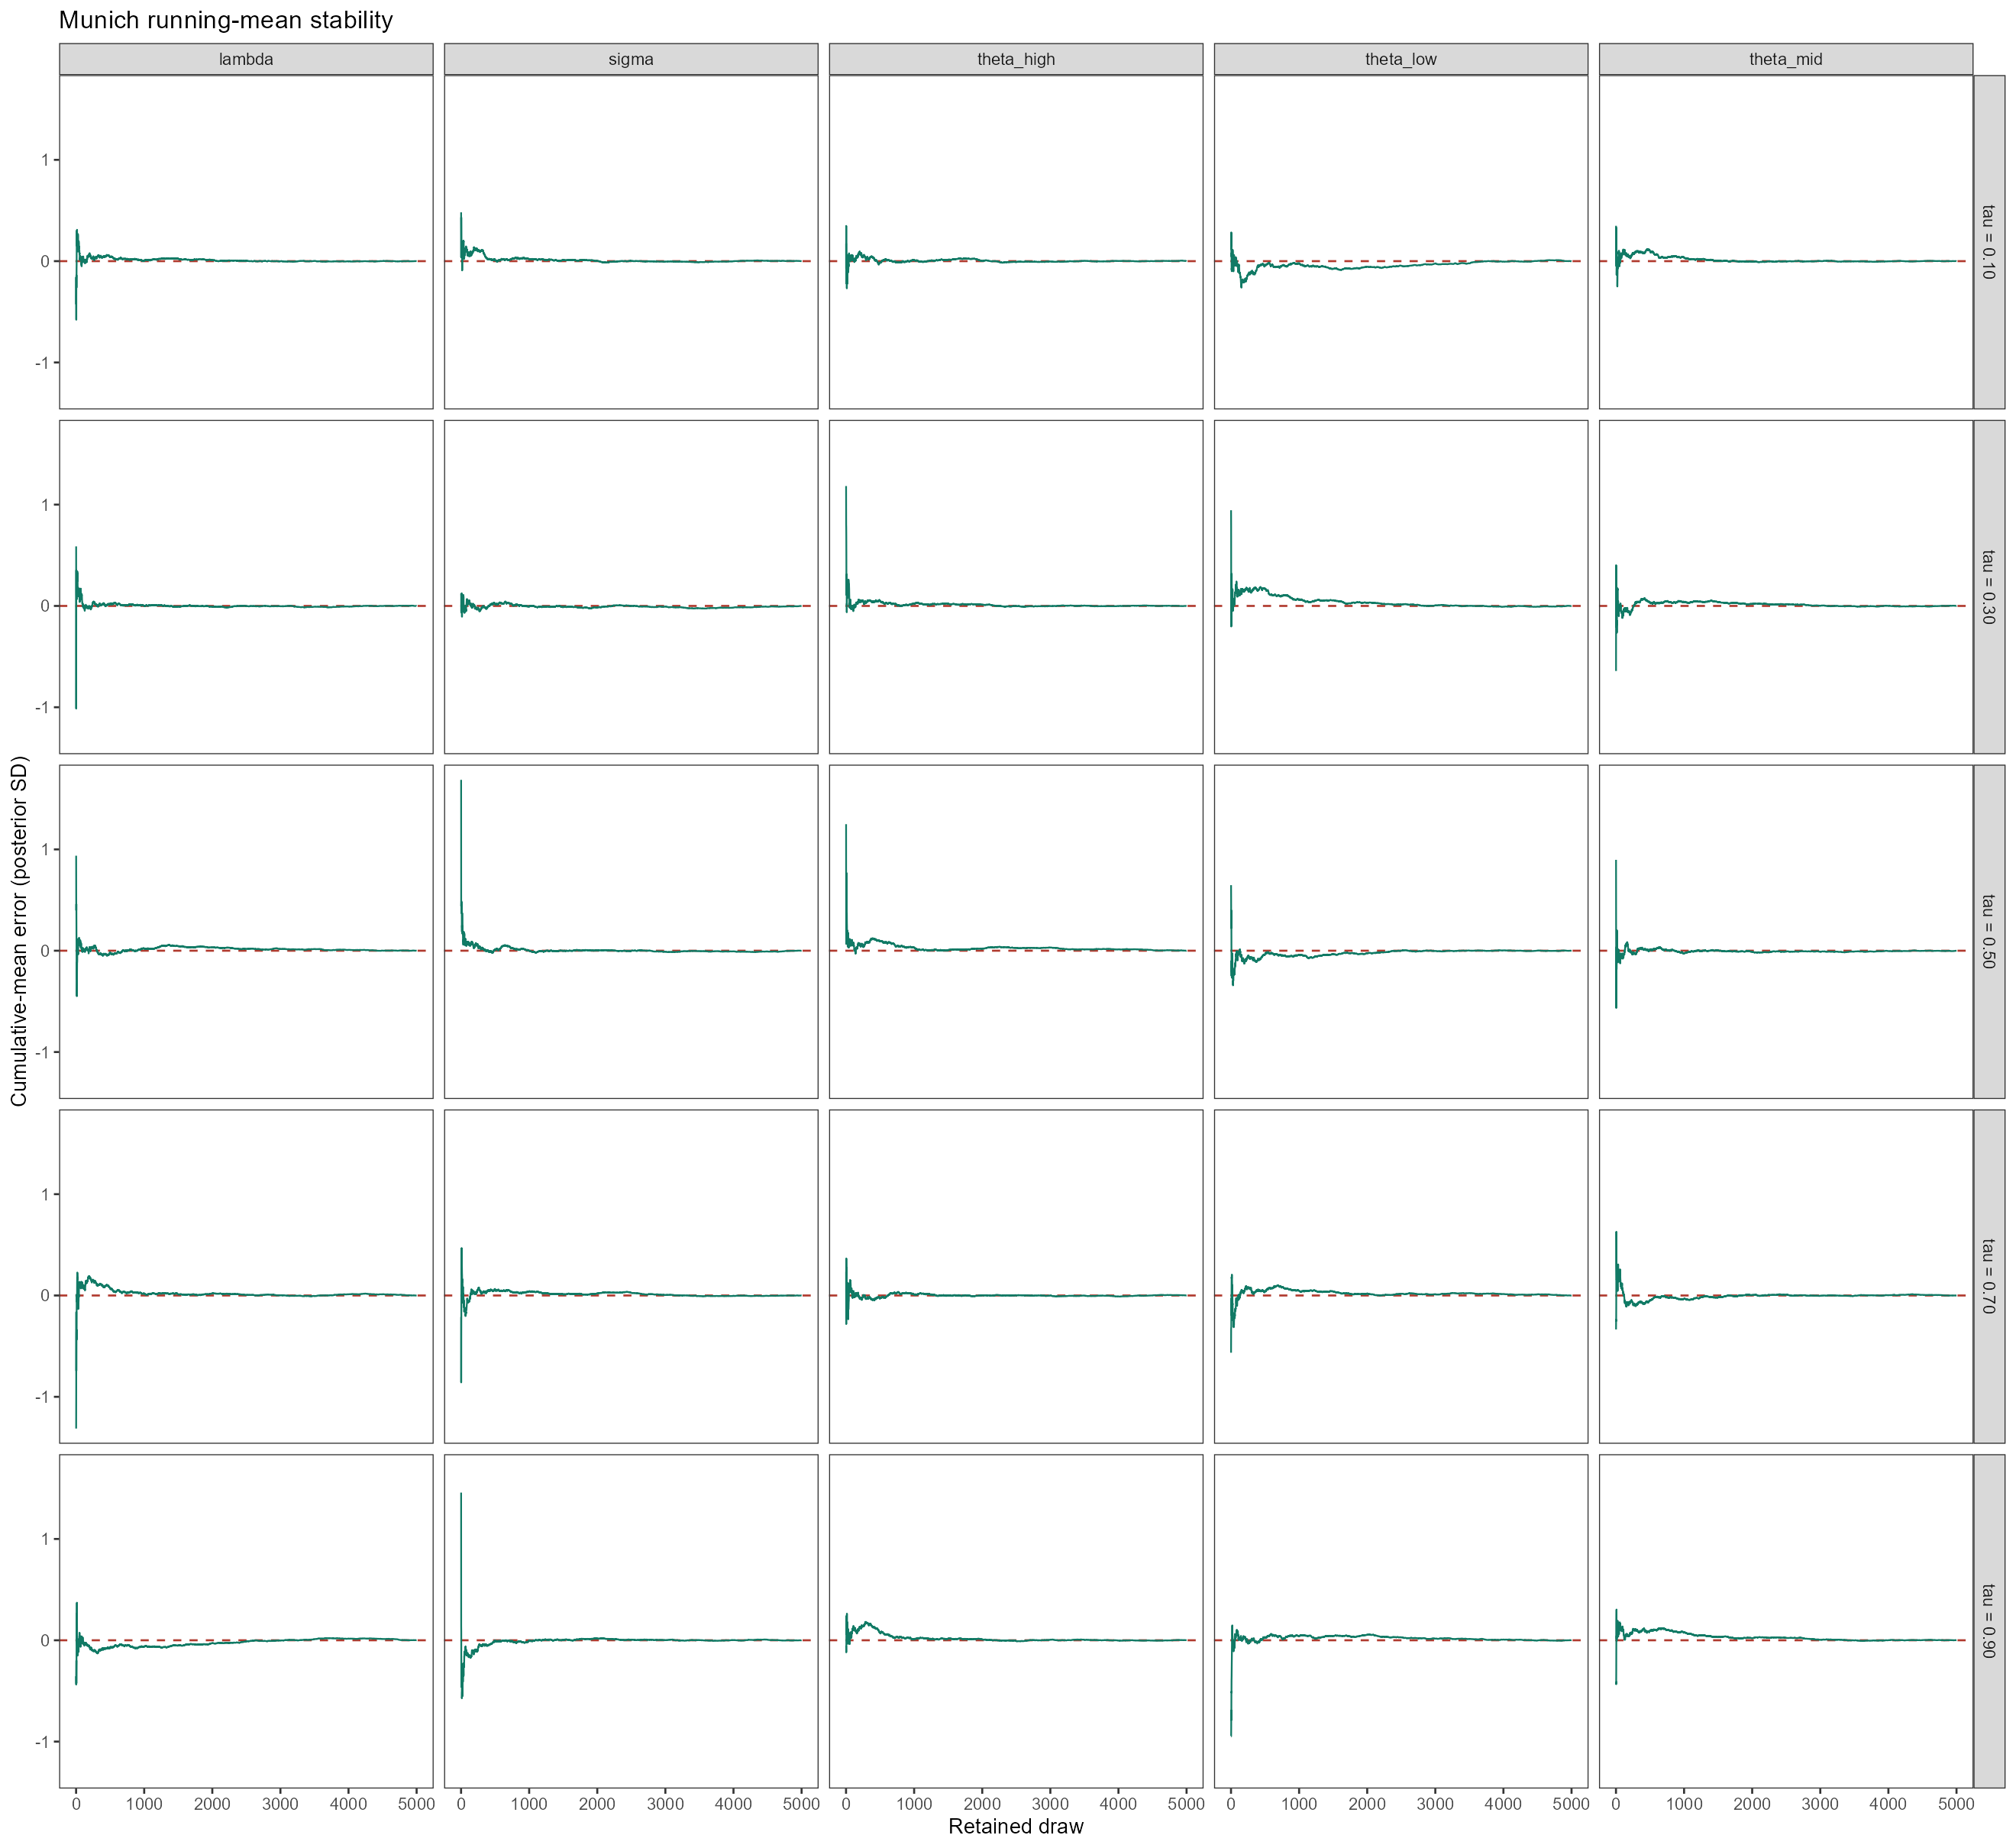
\includegraphics[width=0.75\textwidth,height=0.88\textheight,keepaspectratio]
	{figures/munich_running_mean_stability}
	\caption{Munich standardized cumulative-mean diagnostics.  The curves
		stabilize near zero, with visibly slower settling for selected
		location-specific trend coefficients.}
	\label{fig:munich_running_mean}
\end{figure}
\fi

\subsection{Growth Centiles}
\label{app:growth}

The remaining growth-chart fits of Section~\ref{sec:app:growth} are collected
here: the individual P-MALA/Gibbs fit for girls, and the LMS centiles
\citep{cole1992smoothing} for boys and girls.  The P-MALA settings are those
of Section~\ref{sec:app:growth} ($k = 2$, $\lambda \sim \mathrm{Gamma}(1,\sqrt{G})$,
6{,}000 iterations, 1{,}000 burn-in, one independent run per level).  The LMS
curves are the $10$th, $30$th, $50$th, $70$th and $90$th centiles of the
fitted Box--Cox Cole--Green distribution evaluated on the same 0.1-year age
grid.

\begin{figure}[htbp]
	\centering
	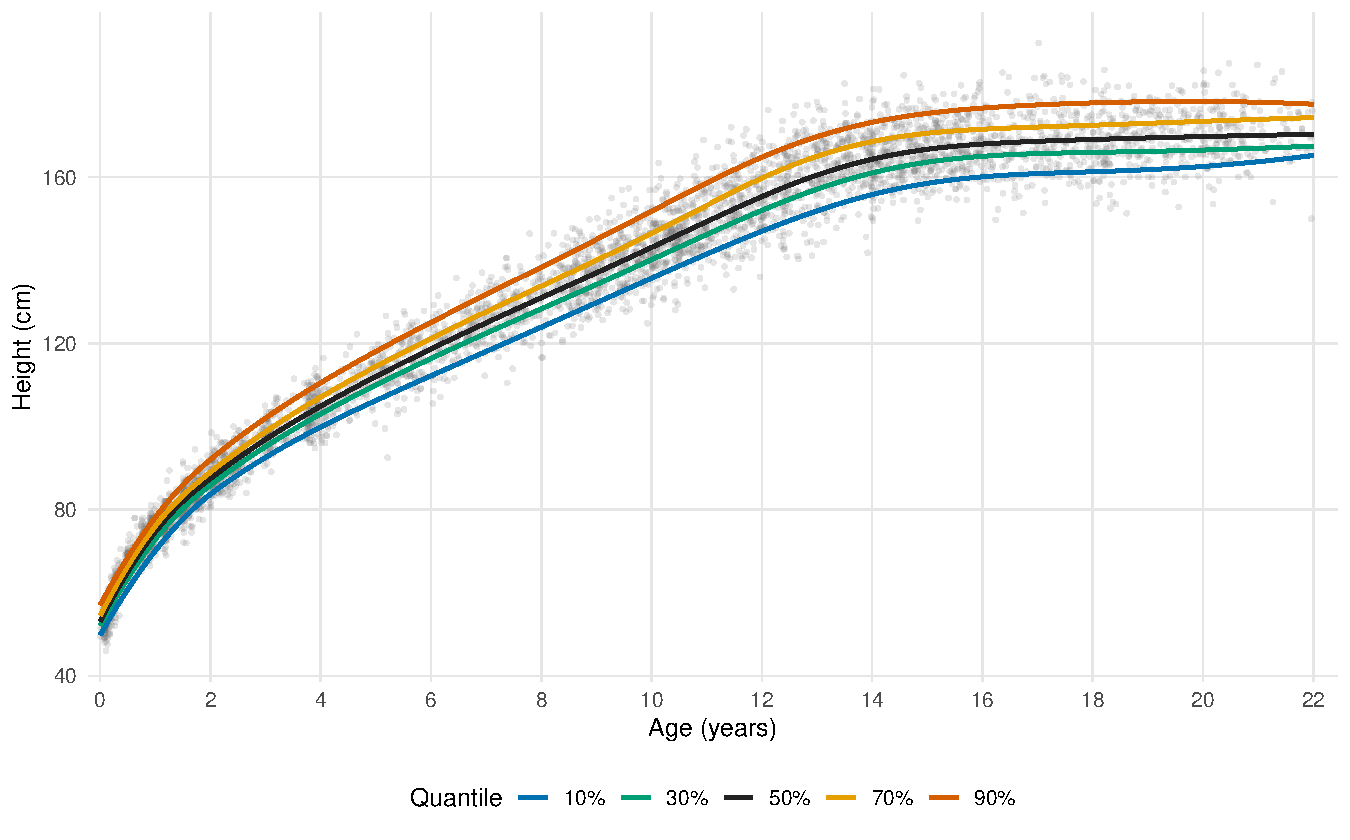
\includegraphics[width=0.75\textwidth]{figures/growth_pmala_girls}
	\caption{Individual P-MALA/Gibbs fits for the height of 5{,}190 Dutch girls
		(Fifth Dutch Growth Study, 2009) at $\tau \in \{0.1, 0.3, 0.5, 0.7, 0.9\}$,
		$k = 2$.  Curves are posterior means; grey circles are the individual
		measurements.}
	\label{fig:growth_girls}
\end{figure}

\begin{figure}[htbp]
	\centering
	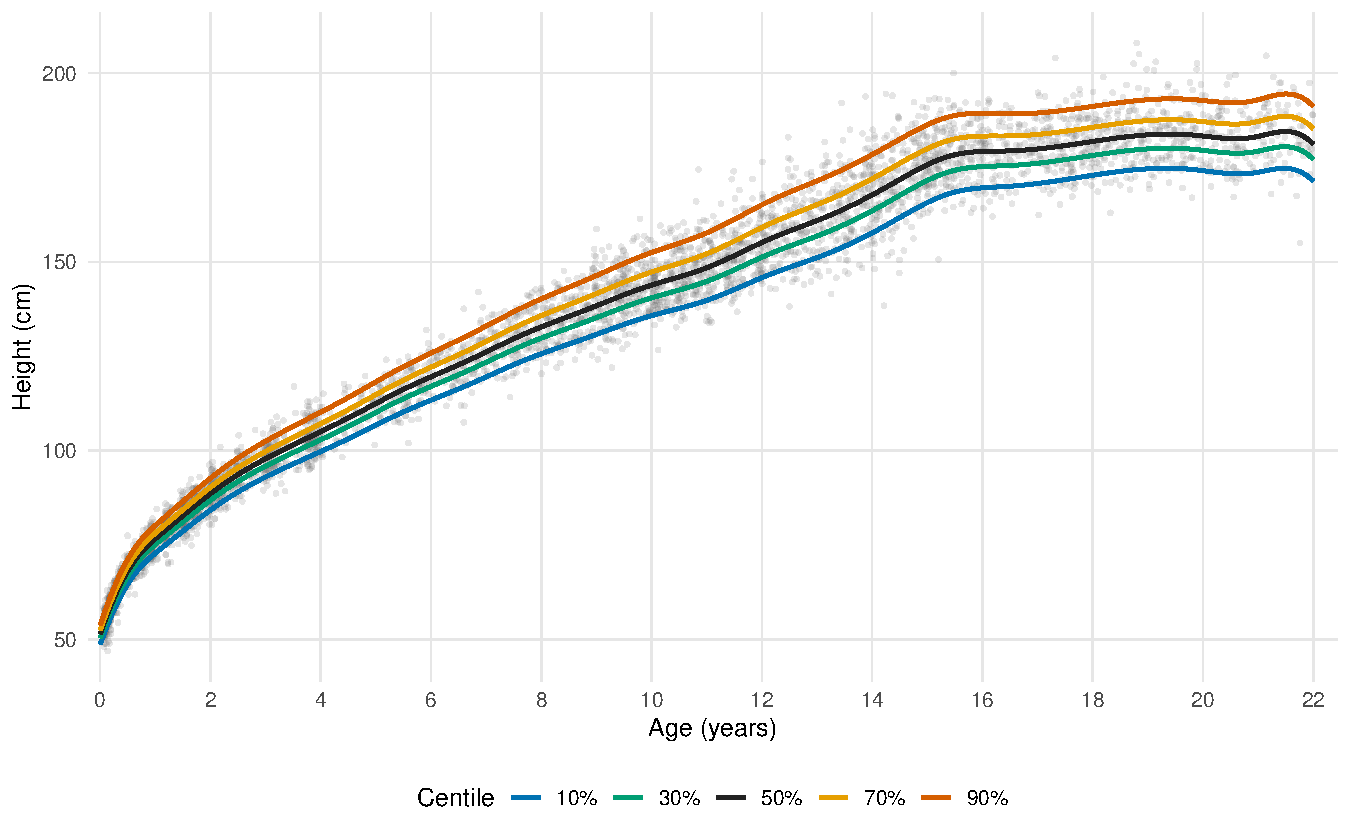
\includegraphics[width=0.75\textwidth]{figures/growth_lms_boys}
	\caption{LMS centiles for the height of Dutch boys: the $10$th to $90$th
		centiles of the fitted Box--Cox Cole--Green distribution, with smooth median,
		coefficient of variation and Box--Cox power in age.}
	\label{fig:growth_lms_boys}
\end{figure}

\begin{figure}[htbp]
	\centering
	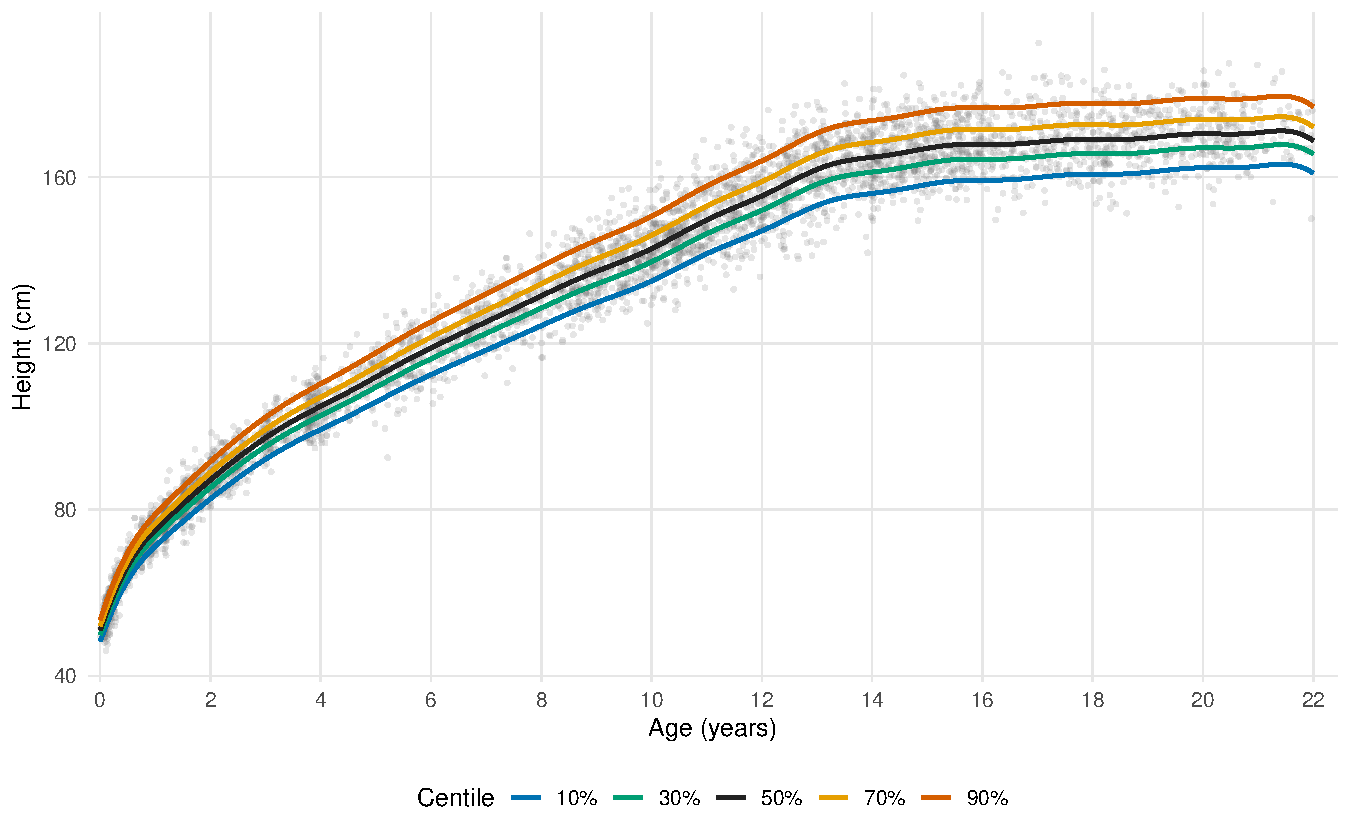
\includegraphics[width=0.75\textwidth]{figures/growth_lms_girls}
	\caption{LMS centiles for the height of Dutch girls, as in
		Figure~\ref{fig:growth_lms_boys}.}
	\label{fig:growth_lms_girls}
\end{figure}